\documentclass[spanish,a4paper,12pt,oneside]{book}

\usepackage[latin1]{inputenc}
\usepackage[T1]{fontenc}
\usepackage[margin=1in]{geometry}
\usepackage{paralist}
\usepackage{graphicx}
\usepackage{url}
\usepackage{times}
\usepackage[spanish]{babel}
\usepackage{listings}
\usepackage{verbatim}
\usepackage{float}
\usepackage{listings}
\usepackage{color}
\usepackage{array}
\usepackage{eurosym}
\usepackage[strict]{chngpage}

\pagestyle{headings}

% El c�digo de estas macros y sus comentarios son obra de Sergio Fern�ndez L�pez (http://www.wikier.org).

%título según la portada oficial de PFC's de la EUITIO
\newcommand{\TituloPFC}{\uppercase{HONOS: Simulador geopol�tico}}
\newcommand{\AutorPFC}{Diego Fern�ndez Fern�ndez}
\newcommand{\DirectorPFC}{Daniel Gayo Avello}

\renewcommand{\maketitle}{
    \begin{titlepage}

	%portada del tomo
	\begin{center}
                {%
                    
\includegraphics[width=3.5cm]{images/uniovi.png}\\
                }
                {%
                    \Large\textrm{\textbf{UNIVERSIDAD DE OVIEDO}}\\
                }
                {%
                    \Large\textrm{Escuela Universitaria de Ingenier�a\\T�cnica en Inform�tica de Oviedo}\\
                    \vspace{4cm}
                }
                {%
                    \Large\textrm{\textbf{PROYECTO FIN DE CARRERA}}\\
                    \vspace{5cm}
                }
                {%
                    \Large\textrm{\TituloPFC}\\
                    \vspace{5cm}
                }
	\end{center}
	\begin{flushright}
		\Large\textrm{\AutorPFC}
	\end{flushright}
	\pagestyle{empty}
	\cleardoublepage

	%portada de dentro
	\begin{center}
                {%
                    \Large\textrm{\textbf{UNIVERSIDAD DE OVIEDO}}\\
                    \vspace{2cm}
                }
                {%
                    
\includegraphics[width=3.5cm]{images/uniovi.png}
                    \hspace{5cm}
                    
\includegraphics[width=3cm]{images/euitio.png}\\
                    \vspace{1cm}
                }
                {%
                    \Large\textrm{ESCUELA UNIVERSITARIA DE INGENIER�A T�CNICA EN INFORM�TICA DE OVIEDO}\\
                    \vspace{3cm}
                }
                {%
                    \Large\textrm{\textbf{PROYECTO FIN DE CARRERA}}\\
                    \vspace{3cm}
                }
                {%
                    \Large\textrm{\TituloPFC}\\
                    \vspace{3cm}
                }
	\end{center}
            {
                \bfseries
                \begin{tabular}{cp{2cm}l}
                \begin{tabular}{|p{5cm}|}
                    \hline
                    \\
                    \\
                    \\
                    {\scriptsize \textbf{V�B� del Director del Proyecto}}\\
                    \hline
                \end{tabular}
		&
		&
                \begin{tabular}{ll}
                        {\footnotesize\textrm\textbf{DIRECTORES:}} &
                        {\textrm\textbf{\DirectorPFC}} \\ &                       
                        \vspace{0.5cm}\\
                        {\footnotesize\textrm\textbf{AUTOR:}} &
                        {\textrm\textbf{\AutorPFC}}
                \end{tabular}
                \end{tabular}
            }
	\pagestyle{empty}
	\cleardoublepage
    \end{titlepage}
}

%cabeceras (con el paquete "fancyhdr")
\headheight 15pt

%macro que me ha chivado Frade, extraido del libro «LaTeX, una imprenta en sus manos», para añadir la bibliografía al indice
\let\OLDthebibliography=\thebibliography
\def\thebibliography#1{\OLDthebibliography{#1}%
	\addcontentsline{toc}{chapter}{\bibname}}

%renombrar las tablas (no funciona)
\renewcommand{\tablename}{Tabla}
\renewcommand{\listtablename}{Indice de tablas}

%colores
\definecolor{darkred}{rgb}{0.5, 0, 0}
\definecolor{violet}{rgb}{1, 0, 1}
\definecolor{green}{rgb}{0.3, 0.95, 0.3}
\definecolor{listinggray}{gray}{0.97}

%listings
\lstset{
	basewidth=0.50em,
	backgroundcolor=\color{listinggray},
	basicstyle=\footnotesize\ttfamily,
	keywordstyle=\bfseries,
	stringstyle=\itshape,
	commentstyle=\itshape,
	showspaces=false,
	showtabs=false,
	showstringspaces=false,
	frame=trbl,
	extendedchars=true,
	numbers=none,
	aboveskip=0.5cm,
	belowskip=0.5cm,
	xleftmargin=0cm,
	xrightmargin=0cm
}

\title{HONOS: Simulador geopol�tico}
\author{Diego Fern�ndez Fern�ndez}
\date{Febrero de 2008}

\begin{document}

\frontmatter

\maketitle

\bibliographystyle{plain}

\chapter*{Agradecimientos}

Quiero expresar mi sincero agradecimiento por la ayuda prestada para la realizaci�n del proyecto a las siguientes personas:
\begin{itemize}
	\item A mi familia por su comprensi�n y paciencia.
	\item A mis amigos por su apoyo e inter�s.
	\item A �ngel Garc�a Voces "`Edy"' por acogerme, por el caf� y, sobre todo, por sus \emph{deja de programar y ponte a dise�ar}.
	\item A Daniel Gayo Avello por la direcci�n y el \emph{inter�s desinteresado}.
	\item A Sonia H. Vazquez por sus dibujos para el interfaz de usuario y por \emph{todo lo dem�s}.
\end{itemize}

\begin{verse}
	\emph{<<Todas las sombras del universo son incapaces de apagar la luz de una peque�a vela>>}
\begin{flushright}
(D.T.Suzuki)
\end{flushright}

\end{verse}

\chapter*{Resumen}

\emph{HONOS: Simulador geopol�tico}, es un juego de estrategia por turnos. En �l, el jugador asume el papel de un presidente de gobierno o primer ministro de un pa�s imaginario y, como tal, deber� hacer frente a una serie de tareas para ganarse el aprecio de su poblaci�n y desarrollar su pa�s. Deber� implementar pol�ticas, mantener relaciones internacionales, cuidar de los servicios p�blicos e intervenir en la producci�n si es necesario.\\

Para ello dispondr� de tiempo y recursos limitados, por su legislatura y por le presupuesto estatal respectivamente. Para ayudar al jugador en esta tarea, dipondr� de datos actualizados sobre el estado de su pa�s y el grado de aceptaci�n de sus pol�ticas entre la gente (dividida en difererentes grupos de poblaci�n con intereses y posiciones sociales variadas ).\\

El �xito o fracaso del jugador depender� de la felicidad que sus ciudadanos acumulen al final de la legislatura.\\

HONOS permite que los jugadores modelen la estructura interna de su pa�s, dando lugar a estados diferentes seg�n su poder econ�mico, las caracter�sticas de los grupos poblacionales que lo componen, la bonanza en le funcionamiento de sus servicios sociales, \ldots mediante ficheros de configuraci�n XML. ESto posibilita que el proyecto, adem�s de un juego, pueda ser una herramienta educativa adaptable por los docentes.\\

La p�gina web del proyecto es \url{http://honos.googlecode.com/}\\

\section*{Palabras clave}
\begin{itemize}
	\item Videojuego
	\item Simulador
	\item Estrategia por turnos
	\item 2D
	\item Configurable
	\item Pol�tica
\end{itemize}


\chapter*{Abstract}
	
\emph{HONOS: geopolitical simulator}, is a turn based strategy game. In it, the player assumes the role of a president of government or prime minister of an imaginary country and, as such, will face a series of tasks in order to earn the esteem of their people and develop their country. It must implement policies, maintain international relations, caring for utilities and intervene in the production if necessary. \\

To do so, will have limited time and resources (the legislature length and state budget). To help the player in this task, it will have an up to date information on the state of his country and the degree of acceptance of its policies among the people (divided into different groups of people with varied interests and social positions). \\

Success or failure will depend on the citizens happiness that its  accumulate at the end of the legislature. \\

HONOS allows players to shape the internal structure of the country, resulting in different states according to their economic power, the characteristics of its population groups, the boom in the functioning of social services, \ldots, through XML configuration files. This makes it possible for the project, in addition to a game, be a customizable educational tool.\\

Project's website at \url{http://honos.googlecode.com/}\\

\section*{Keywords}
\begin{itemize}
	\item Videogame
	\item Simulator
	\item Turn based strategy
	\item 2D
	\item Customizable
	\item Politics
\end{itemize}

\chapter*{Licencia}

\section*{Documento}

El contenido de este documento se encuentra protegido por la licencia 
\emph{Creative Commons Reconocimiento-Compartir bajo la misma licencia 2.5 Espa�a} (anexo \ref{sec:license.cc}).

%\section*{C�digo fuente}
%
%El c�digo fuente (disponible en el anexo \ref{sec:source}) se encuentra 
%licenciado bajo la licencia \emph{GNU General Public License (GPL)}, 
%versi�n 2 o superior (anexo \ref{sec:license.gpl}).

\tableofcontents

\newpage

\listoffigures

\newpage

\listoftables

\newpage

\mainmatter

\chapter{Introducci�n}
\label{sec:introduccion}

\section{Justificaci\'on del proyecto}
\label{sec:justificacion}

A d\'{\i}a de hoy, la creaci\'on profesional de videojuegos supone uno de los mayores retos a los que se puede enfrentar un profesional de la inform\'atica: los videojuegos de \'ultima generaci\'on llevan al l\'{\i}mite los requisitos hardware de los ordenadores personales en aras del realismo y el entretenimiento, suponen el trabajo de grandes equipos de desarrollo durante per\'{\i}odos de tiempo que no bajan de los tres a\~nos, los presupuestos que se manejan para su creaci\'on y distribuci\'on igualan a los de las grandes producciones cinematogr\'aficas y los beneficios que reportan empiezan a superar a otros medios de entretenimiento m\'as tradicionales.\\

La industria de los videojuegos demanda profesionales con una amplia formaci\'on y una gran motivaci\'on con la promesa, no de unos grandes sueldos, si no la de desarrollar un trabajo que muchas veces anda a medio camino entre la ingenier\'{\i}a y el arte, entre la t\'ecnica y la imaginaci\'on.\\

Al igual que el resto de medio de comunicaci\'on los videojuegos no s\'olo pueden representar una alternativa de ocio: las experiencias del jugador y los mensajes m\'as o menos expl\'{\i}citos pueden ser (y de hecho son) utilizados con fines docentes o sociales. Cada vez son m\'as lo ejemplos de videojuegos que son introducidos en las aulas para reforzar conceptos pedag\'ogicos o para concienciar sobre alguna realidad actual (cambio clim\'atico, conflictos armados, inmigraci\'on, etc).\\

Para entrar en el negocio del entretenimiento electr\'onico, al menos desde la perspectiva de la creaci\'on, es casi imprescindible acompa\~nar un curr\'{\i}culum vitae con una muestra del trabajo que el aspirante ha sido capaz de realizar, generalmente en forma de juego m\'as o menos completo.\\

As\'{\i} pues, HONOS nace con una doble pretensi\'on: la de acompa\~nar un curr\'{\i}culum de alguien que querr\'{\i}a ganarse la vida con esta profesi\'on, y la de poner un granito de arena m\'as al reconocimiento de los videojuegos como un poderoso medio de comunicaci\'on, educaci\'on y concienciaci\'on.\\

\newpage
\section{Objetivos del Proyecto}
\label{sec:objetivos}

Los objetivos del proyecto se pueden dividir en dos grandes categor�as, una en relaci�n a los requisitos t�cnicos que impone la especificaci�n del proyecto y otra que atiende a las necesidades de formaci�n para poder ser un trabajador en la industria de los videojuegos.

As� pues, a nivel t�cnico los objetivos del proyecto son:
\begin{itemize}
	\item Desarrollar un juego completo.
	\item Conseguir que este cumpla los objetivos planteados en el apartado de an�lisis.
\end{itemize}

A nivel pedag�gico:
\begin{itemize}
	\item Conseguir un grado aceptable de capacitaci�n en el manejo de diversas tecnolog�as demandadas por la industria.
	\item Poner en pr�ctica diferentes conocimientos que se supone se han adquirido durante el estudio de la carrera.
	\item Mejorar y ampliar dichos conocimientos.
\end{itemize}
\newpage
\section{Estudio de la situaci\'on actual}
\label{sec:estado-actual}

\subsection{Precursores: juegos de tablero.}

Los juegos de estrategia por turnos han estado presentes en la civilizaci\'on desde hace m\'as de 4000 a\~nos. Probablemente los m\'as representativos sean, precisamente, los m\'as antiguos: el tradicional Go chino, que ya se practicaba 2000 a\~nos antes del nacimiento de Cristo, o el ajedrez. Ambos fueron considerados durante siglos mucho m\'as que simples entretenimientos y en la antigua civilizaci\'on china la maestr\'{\i}a en el Go supon\'{\i}a la mejor muestra de erudici\'on de un hombre culto.\\

\begin{figure}[h]
	\centering
		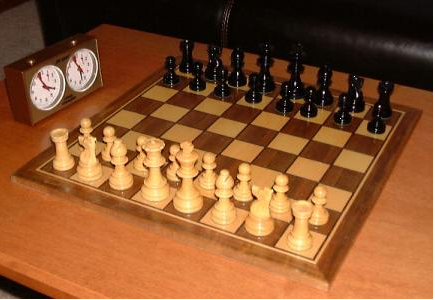
\includegraphics[width=10cm]{images/ajedrez.png}
	\caption{Juego de ajedrez tradicional}
	\label{fig:ajedrez}
\end{figure}

\begin{figure}[h]
	\centering
		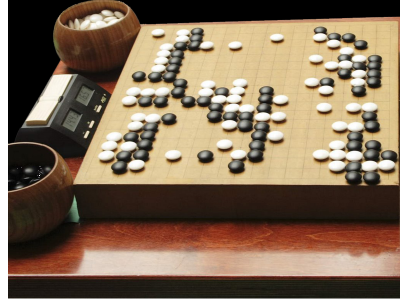
\includegraphics[width=10cm]{images/go.png}
	\caption{Juego de ajedrez chino tradicional o Go}
	\label{fig:go}
\end{figure}

Fij\'andonos en estos dos representantes primigenios de los juegos de estrategia por turnos se puede dar una definici\'on del conjunto: Un juego de estrategia por turnos es aquel en el cual los jugadores disponen de tiempo para meditar su siguiente movimiento (su turno) y que finaliza cuando se realiza dicho movimiento. Es decir en contraposici\'on a los juegos de estrategia en tiempo real, \emph{la acci\'on} se detiene entre cada jugada.
\\
Con estas simples premisas existen infinidad de ejemplos de juegos de tablero que cumplen con esta definici\'on y que son m\'as o menos conocidos: 
\begin{itemize}
	\item \emph{El Risk} se juega sobre un tablero que representa un mapamundi, sobre el los jugadores despliegan fichas que representan sus ej\'ercitos, el objetivo del juego es conquistar una serie de territorios a otros jugadores.
	\item \emph{El Scrabble} es un juego cuyo objetivo consiste en formar palabras sobre un tablero. Para dicho fin, cada jugador recibe un n\'umero espec\'{\i}fico de fichas (o letras), las cuales debe colocar sobre casillas numeradas. Las letras se encuentran igualmente numeradas, y por lo tanto, cada jugador obtiene por cada palabra formada un puntaje que depende tanto del valor de las letras empleadas como de la posici\'on de dichas letras dentro del tablero.
	\item \emph{El Reversi} es un juego entre dos personas, que comparten 64 fichas iguales, de caras distintas, que se van colocando por turnos en un tablero dividido en 64 escaques. Las caras de las fichas se distinguen por su color y cada jugador tiene asignado uno de esos colores, ganando quien tenga m\'as fichas sobre el tablero al finalizar la partida.
\end{itemize}

\subsection{Salto al mundo digital: estrategia por turnos en el PC.}

Los primeros juegos de estrategia por turnos para ordenador fueron, como era de esperar, adaptaciones de los antiguos juegos de tablero. Los retos t\'ecnicos de estos proyectos  se encontraban sobre todo en el apartado de la simulaci\'on y la inteligencia artificial, es decir, en la capacidad de dise\~nar e implementar un sistema que fuera capaz de comportarse como uno o varios jugadores a los que el usuario pudiera enfrentarse. Como an\'ecdota al respecto cabe destacar la \textit{moda} que durante la d\'ecada de los 90 enfrent\'o a superodenadores contra grandes maestros del ajedrez, siendo los m\'as famosos los enfrentamientos entre Gary Kasparov y la computadora de IBM Deep Blue. Actualmente, en cuanto a computaci\'on y ajedrez se refiere se opta por soluciones m\'as enfocadas al software que al hardware (como era Deep Blue) y programas que se pueden encontrar en las estanter\'{\i}as de de las tiendas de videojuegos han sobrepasado el rendimiento de Deep Blue de manera m\'as que notable.\\

\begin{figure}[h]
	\centering
		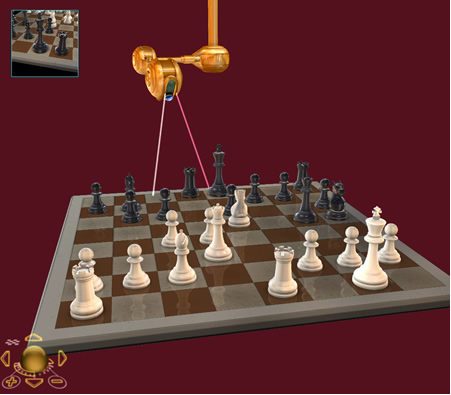
\includegraphics[width=10cm]{images/fritz11.png}
	\caption{Fritz 11, Frans Morsch and Mathias Feist (2007)}
	\label{fig:Imagen de Fritz 11}
\end{figure}
 
Un claro ejemplo de esto es el programa alem\'an Fritz. Por menos de 50 euros cualquiera puede tener en casa un software que ha demostrado su val\'{\i}a derrotando al campe\'on mundial Vladimir Kramnik\footnote{En realidad el programa que venci\'o fue Deep Fritz, una versi\'on optimizada para el uso de procesadores multi-n\'ucleo.}.\\

Pero el medio que brinda el ordenador, m\'as libre de ciertas ataduras f\'{\i}sicas inherentes a los juegos de tablero, pronto comenz\'o a dar como resultado nuevas y m\'as ricas formas de entretenimiento basadas (aun as\'{\i}) en los mismos principios que sus antecesores.\\

Quiz\'as el exponente m\'as claro y con mayor repercusi\'on de la estrategia por turnos dentro del entretenimiento digital sea el \emph{Civilization} de Sid Meier, cuya primera versi\'on data de 1991.\\

\begin{figure}
	\centering
		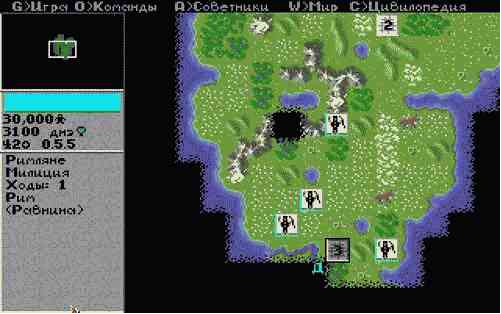
\includegraphics[width=10cm]{images/civilization.png}
	\caption{Civilization, Sid Meier (1991)}
	\label{fig:Imagen de la primera versi\'on para DOS del Civilization}
\end{figure}	
	
En Civilization el jugador toma el rol del regente de una civilizaci\'on empezando con una simple unidad-poblador y trata de construir un imperio compitiendo con otras civilizaciones.\\

El objetivo del juego es dirigir esta civilizaci\'on desde su inicio hasta llegar al espacio o conquistar todo el planeta. Permite ir decidiendo el camino que toman las investigaciones cient\'{\i}ficas,  se puede fundar ciudades, construir y comandar ej\'ercitos, dirigir la construcci\'on de carreteras, elegir la forma de gobierno, mantener relaciones diplom\'aticas con otros pueblos, etc.\\

Existen gran cantidad de versiones de este juego en forma de secuelas oficiales, adaptaciones o incluso una versi\'on completamente libre llamada \emph{FreeCiv}.\\

A partir del Civilization surgieron multitud videojuegos que tomando el concepto trasladaron la acci\'on al espacio exterior (\emph{Master of Orion}, \emph{Ascendancy}), a mundos de fantas\'{\i}a (\emph{Heroes Of Might and Magic}) o a per\'{\i}odos hist\'oricos concretos (\emph{Pirates!}).\\

\subsection{La pol\'{\i}tica en los videojuegos}

Si bien es cierto que el Civilization y sus derivados conten\'{\i}an una gran parte de gesti\'on, su mec\'anica y sobre todo las condiciones del jugador para ganar, exig\'{\i}an que las actividades pol\'{\i}ticas que se pudieran realizar fueran bastante limitadas. En cualquier caso, el objetivo del juego no era el de simular la actividades de un l\'{\i}der pol\'{\i}tico.\\

Para encontrar un juego as\'{\i} tenemos que remontarnos todav\'{\i}a m\'as atr\'as en el tiempo, hasta 1988 con el videojuego \emph{Hidden Agenda}.\\

\begin{figure}[h]
	\centering
		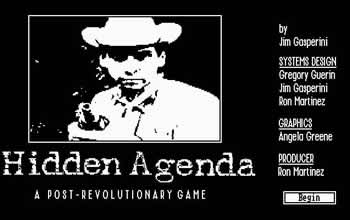
\includegraphics[width=10cm]{images/hiddenAgenda.png}
	\caption{Hidden Agenda, Jim Gasperini (1988)}
	\label{fig:Pantalla inicial de Hidden Agenda}
\end{figure}		
	
En \'el, el jugador asume el papel de un reci\'en electo presidente de un pa\'{\i}s imaginario de Am\'erica latina, reci\'en salido de un r\'egimen dictatorial. La mayor parte del juego se basa en leer textos sobre consejeros pertenecientes a diferentes facciones y tomar decisiones con respecto a estas, tratando de mantener contenta a la mayor parte de la poblaci\'on representada por dichas facciones. Exist\'{\i}a un m\'{\i}nimo componente geopol\'{\i}tico que se manifestaba en la capacidad la alinearse con alguna potencia internacional (EEUU, antigua Uni\'on Sovi\'etica y Europa). Se le considera uno de los precursores del movimiento GamesForChange\footnote{Games for Change (tambi\'en conocido como G4C) es un movimiento y comunidad dedicado al uso de los videojuegos como elemento de cambio social. Se puede encontrar m\'as informaci\'on en us we: http://www.games4change.org }.\\

El ejemplo m\'as contempor\'aneo de juego relacionado con la gesti\'on pol\'{\i}tica es \emph{Democracy}: creado en 2005, el jugador asume el papel de presidente/primer ministro de un gobierno democr\'atico. Las funciones del jugador consisten en introducir y alterar pol\'{\i}ticas en siete areas diferentes (impuestos, econom\'{\i}a, bienestar, relaciones externas, transporte, ley y orden y servicios p\'ublicos). Cada pol\'{\i}tica tienen un efecto en la felicidad de diferentes grupos de poblaci\'on, as\'{\i} como en factores como el crimen o la poluci\'on del aire. 

\begin{figure}[h]
	\centering
		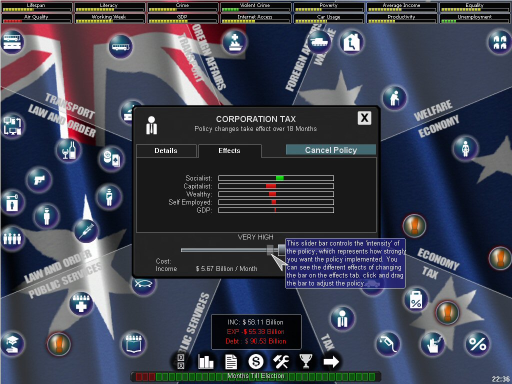
\includegraphics[width=10cm]{images/democracy.png}
	\caption{Democracy, Positech Games (2005)}
	\label{fig:Pantalla de juego de Democracy}
\end{figure}

En principio Democracy puede ser el juego que m\'as  se parezca a HONOS en su planteamiento y concepci\'on. Las diferencias fundamentales radican en que en HONOS se hace mayor hincapi\'e en la intervenci\'on m\'as directa del jugador en ciertos aspectos y no s\'olo a base de pol\'{\i}ticas, as\'{\i} como una mayor complejidad en las relaciones diplom\'aticas.

\chapter{Aspectos te�ricos}
\label{sec:aspectos-teoricos}

\section{Modelado del pa�s}
Como toda simulaci�n HONOS trata de plantear un modelo m�s o menos formal de los diferentes aspectos con los que juega: poblaci�n, producci�n, servicios sociales, diplomacia etc. A continuaci�n se expone a grandes rasgos las diferentes aproximaciones dise�adas e implementadas para dotar al programa del grado de verosimilitud deseado.

\subsection{Nivel de vida}
Se considera el nivel de vida del estado a simular como un conjunto de factores que formalizan la \emph{felicidad} de la poblaci�n. Esta va a ser la medida que, en definitiva, decida el �xito del jugador en su papel de presidente. Sin embargo existe una complejidad conceptual a la hora de decidir como calcular el nivel de vida. Las dificultades que se plantean son las mismas que ocurren en el mundo real y est�n relacionadas con la ambig�edad y subjetividad inherente al t�rmino bienestar.\\
 
Centr�ndose en lo que s� puede ser medible, se puede calcular esta magnitud atendiendo a los siguientes puntos:
\begin{itemize}
	\item Satisfacci�n de las necesidades de consumo.
	\item Actividad pol�tica.
	\item Relaciones internacionales.
	\item Existencia de conflictos armados (terrorismo, guerras civiles, guerras con otros estados, \ldots). 
	\item Calidad de los servicios p�blicos.
\end{itemize}

\subsection{Poblaci�n}
La poblaci�n se distribuye en diferentes grupos. De cada uno de ellos se establece la importacia que dan a los factores que condicionan el nivel de vida expuestos anteriormente. As� pues, de cada grupo se puede definir la importancia que consideran sobre dichos aspectos.\\

Tambi�n se define otro conjunto de caracter�sticas necesarias para la simulaci�n:

\begin{itemize}
	\item Tama�o del grupo. Define el porcentaje de poblaci�n del total que corresponde al grupo en cuesti�n.
	\item Poder adquisitivo. Define el porcentaje de la riqueza total del pa�s que tiene cada grupo. Definir� en que medida es afectado por las variaciones de precio en los productos de consumo como se ver� en la secci�n \ref{sec:consumo}.
\end{itemize}

\subsubsection{Consumo}
\label{sec:consumo}
Para satisfacer las necesidades de consumo con respecto a la producci�n, la importacia que le hayamos otorgado y el tama�o del grupo de poblaci�n, se implementa un modelo matem�tico que nos indica cual es la reacci�n ante los cambios de precio en los diferentes productos. Utilizando una funci�n de la forma $1- x ^{\lg{1 - poder adquisitivo}/\lg{0.5}}$ obtenemos curvas que representan el acceso a un producto con una cierta inflacci�n seg�n el poder adquisivo del mismo.\\

Por ejemplo, para un grupo de poblaci�n que acapara el 70\% de la riqueza del pa�s, tendremos una funci�n como esta:
\begin{figure}[h]
	\centering
		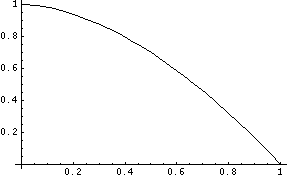
\includegraphics[width=10cm]{images/plot2D.png}
	\caption{Gr�fica de consumo 2}
	\label{fig:Eje x cambios de precio. Eje y consumo}
\end{figure}

Sin embargo, para un grupo de poblaci�n que acapara el 30\% de la riqueza del pa�s, tendremos una funci�n como esta:
\begin{figure}[h]
	\centering
		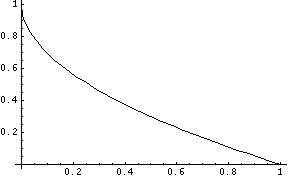
\includegraphics[width=10cm]{images/plot2D2.png}
	\caption{Gr�fica de consumo 2}
	\label{fig:Eje x cambios de precio. Eje y consumo}
\end{figure}

Podemos constatar como, a menor riqueza, una variaci�n de precios supone una p�rdida de capacidad adquisitiva mucho m�s pronunciada.\\

As� podemos observar que se modela bastante bien el comportamiento de los distintos grupos de poblaci�n seg�n su capacidad de consumo: cuanta m�s riqueza acaparan, menos sensibles son los cambios de precio y por lo tanto tienen mayor margen para satisfacer sus necesidades de consumo. Lo contrario ocurre con los grupos cuyo poder adquisitivo sea m�s bajo.\\

Esto, combinado con la importancia que cada grupo le otorga al consumo nos permite modelar de una forma l�gica el comportamiento de una sociedad heterogenea.

\subsection{Producci�n}
Al usuario no se le muestran la mayor parte de los datos con los que trabaja internamente producci�n, por una parte para no atosigarlo con cifras y por otra porque el conocimiento como presidente del gobierno de los pormenores productivos de la naci�n es limitado, as� como su capacidad de intervenci�n.\\

Internamente, producci�n trabajo con el modelo m�s simple de mercado: el de la oferta y la demanda. Sin embargo se le ha dotado de otros mecanismos que permiten a la producci�n evolucionar de forma autom�tica siguiendo dos simples normas:

\begin{itemize}
	\item Tratar de satisfacer siempre la demanda.
	\item Tratar de maximizar los beneficios.
\end{itemize}

En resumen producci�n es un ente con el que el jugador se relaciona directamente de forma limitada, pero que afecta en gran medida el desarrollo del juego. Por eso debe comportarse de forma \emph{aparentemente} inteligente y aut�noma.

\subsection{Servicios sociales}
A nivel b�sico los servicios sociales afectan a la felicidad de la poblaci�n seg�n su funcionamiento. La percepci�n que estos tienen de dicho funcionamiento se mide en HONOS mediante la \emph{calidad}: cuanta mayor calidad tiene un servicio m�s contenta est� la poblaci�n con �l.\\

En la vida real influyen infinidad de par�metros sobre dicho funcionamiento; para esta simulaci�n se han tomado dos: los recursos humanos y los recursos materiales. La raz�n es que, de la forma que se comentar� m�s adelante, estos par�metros pueden ser contrastados y comparados con valores de calidad seg�n estipulan diversas organizaciones internacionales.\\

No s�lo afecta la cantidad de estos dos recursos, si no la productividad de los mismos. Para medir esto nos valemos otra vez una funci�n matem�tica de forma a la anteriormente mencionada para consumo. De esta forma obtenemos un i�ndice de productividad en funci�n del recurso y el dinero invertido en el.

\subsection{Diplomacia}
Las relaciones diplom�ticas se basan en establecer tratados con las diferentes naciones con las que tenemos relaci�n. El concepto clave en este caso es \emph{opini�n}: dependiendo de la opini�n que la potencia extranjera tenga sobre nuestro pa�s podremos hacer a m�s o menos tratados con esta.\\

Cada uno de estos compromisos supone unos beneficios e inconvenientes que se manifiestan en diversos par�metros de la simulaci�n: desde la producci�n hasta la felicidad de un grupo poblacional. Pero, adem�s de los efectos causados, cada tratado tiene unos requisitos que debemos de satisfacer; la �ndole de estos tambi�n puede ser diversa: desde el estado de nuestros servicios sociales, hasta los precios de exportaci�n de nuestros productos. As� pues si la opini�n del pa�s con el que queremos mantener relaciones es suficiente y cumplimos los requisistos para un tratado concreto, podremos iniciar �ste y se mantendr� siempre y cuando los requisitos antes mencionados se mantengan dentro de unos par�metros razonables.\\

\section{Opciones de personalizaci�n}
En cierta medida HONOS est� construido para que pueda ser modificado adapt�ndolo a los gustos o necesidades del jugador a la hora de simular una realidad nacional diferente. As� pues multitud de par�metros son personalizables mediante ficheros de configuraci�n. As� pues, el juego permite configurar los siguientes aspectos:

\begin{itemize}
	\item Lista de pol�ticas, con sus requerimientos y sus efectos.
	\item Lista de tratados, con sus requerimientos y sus efectos.
	\item Estados iniciales de la producci�n y los servicios sociales (�c�mo funcionaban estos antes de nuestra elecci�n como presidente?)
	\item Distribuci�n de la riqueza. Podemos definir en que medida se distribuye la riqueza entre lso diferentes grupos de poblaci�n.
	\item Distribuci�n poblacional. Podemos definir en que medida se distribuye la poblaci�n entre los diferentes grupos.
	\item Niveles de importancia. Podemos definir en que manera afecta cada par�metros de nuestro pa�s a cada grupo poblacional.
	\item Costes y sueldos. Podemos definir cual es gasto �ptimo en recursos para los diferentes servicios sociales.
	\item Definic�n de calidad de servicios. Podemos definir (dentro del binomio recursos humanos - recursos materiales) que cantidad de estos se consideran �ptimos.
\end{itemize}

\section{Immediate Mode Graphic User Interface (IMGUI)}
\label{sec:imgui}
Immediate Mode Graphic User Interface (IMGUI) es una nueva aproximaci�n a la implementaci�n de interfaces gr�ficas de usuario (\emph{GUIs}). La forma m�s sencilla de explicar en que consiste es por contraposici�n con la forma \emph{estandar} de implementar GUIs: la forma m�s extendida se basa en poner los componentes del GUI en pantalla, preguntarles por su estado y enviar mensajes.\\

Dicho intercambio de informaci�n se realiza mediante eventos que los componentes \emph{escuchan} y reaccionan de forma apropiada. Una vez finalizado su uso, como es normal, los componentes se eliminan y se liberan sus recursos.\\

Todo esto conlleva en la pr�ctica definir muchas lineas de c�digo para implementar la funcionalidad m�s simple de, pongamos un bot�n. Adem�s dicho c�digo, aunque muy acorde con el paradigma de la orientaci�n a objetos, rompe la estructuraci�n lineal del flujo del programa: normalmente donde se produce un evento, se captura y se procesa, es un lugar diferente y en muchos casos poco transparente.\\

Lo que se trata de conseguir con IMGUI son, principalmente dos objetivos:

\begin{enumerate}
	\item En primer lugar simplificar la implementaci�n de los GUIs logrando resultados de forma m�s r�pida e intuitiva.
	\item Conseguir que el flujo del programa \emph{viaje} por el interfaz de usuario de forma m�s lineal (aunque esto suponga un paso hacia la programaci�n estructurada que los purista de la orientaci�n a objetos pueden no ver con buenos ojos).
\end{enumerate}

IMGUIs tienen sus contras, pero a la hora de realizar GUIs para aplicaciones en tiempo real (como por ejemplo juegos) sus ventajas priman: los componentes son renderizados y utilizados justo en el sitio donde se necesitan y son llamados de forma clara en el c�digo.\\

Para todo esto es necesario tener una biblioteca de componentes que permita reproducir este comportamientos (esa es una de las razones por las que para este proyecto se ha dise�ado e implementado una desde cero). Una parte importante de esta biblioteca es procurar una forma en la que el \emph{estado} del interfaz sea compartido por todos los componentes y no sean estos los que lo almacenen.\\

Un estado global para todos los componentes no es una idea descabellada, en la mayor parte de los casos (en todos, en lo que a este proyecto se refiere) par�metros como el foco, la posici�n del rat�n, etc, s�lo tienen sentido referidos a un componente en un momento de tiempo dado, es decir: por cada frame s�lo se puede interactuar con un componente.\\

Las caracter�sticas de la implementaci�n espec�fica para la biblioteca de componentes gr�ficos de este proyecto son:
\begin{itemize}
	\item Existe una estructura �nica compartida por todos los componentes que almacena la informaci�n de \emph{interacci�n} en cada momento (posici�n del rat�n, foco, estado del componente con el foco, etc).
	\item El componente con el que se interactua puede estar en dos estados: uno modela el estado en que estamos a punto de interactuar con �l (o al menos tenemos esa posibilidad) y otro que indica que estamos interactuando con �l.
	\item En un momento determinado s�lo un componente de cada vez puede estar en alguno de los dos estados.
	\item Los eventos generados por el usuario mediante su iteraci�n (movimiento del rat�n, pulsaci�n de botones, etc) s�lo son enviados a un elemento: aquel que est� en uno de los dos estados susceptibles de ser interactuados.	
\end{itemize}

Durante el dise�o del GUI para HONOS surgi� un problema del que no se habla en la poca documentaci�n que hay al respecto de los IMGUIs: \emph{�qu� sucede en los casos en los que se interactua con dos elementos al mismo tiempo?} La respuesta es simple: eso no puede suceder.\\

Antes de explicar la soluci�n, tratar� de exponer el problema con un ejemplo clarificador: dos componentes superpuestos comparten, como m�nimo, algo de su area. Cuando interacionamos con ese area compartida se produce un conflicto, �con qu� elmento estamos interactuando? El sentido com�n nos dice que nuestra intenci�n siempre ser� interactuar con el componente que ocupe la posici�n superior.\\

Por ello la biblioteca utilizada almacena no s�lo la posici�n en dos dimensiones (como es natural en un iterfaz 2D) sino tambi�n el nivel (o posici�n Z) en el que se encuentra.

\section{Resource Adquisition Is Initialization (RAII)}
\label{sec:raii}
Resource Adquisition Is Initialization (RAII) es un patr�n de dise�o muy usado en lenguajes como ADA, D y C++. Basicamente consiste en asegurar que la adquisici�n de recursos se producir� en la inicializaci�n de los objetos y de forma at�mica. De la misma forma este patr�n trata de asegurar que la destrucci�n de los mismos conllevar� la liberaci�n de los recursos asignados en su construcci�n.\\

En C++ y para asegurarnos la contrucci�n de objetos siguiendo este patr�n hacemos uso de los denominados \emph{punteros inteligentes}: creamos los objetos con el operador \emph{new} y asignamos el puntero resultante a un puntero inteligente. Cualquier fallo en la inicializaci�n de recursos (lo que se traduce a cualquier fallo en la construcci�n de un objeto) resulta en una excepci�n que, en principio, nos hace perder el flujo de ejecuci�n esperado. Los punteros inteligentes se encargan autom�ticamente de eliminarse a la salida de su �mbito por lo que no debemos preocuparnos por que una excepci�n propicie esto.\\

Una vez creados todos los recursos necesarios y asignados a punteros inteligentes, si no se ha habido ning�n error, tenemos un objeto perfectametne construido y con sus recursos asignados correctamente. Para evitar que estos se pierdan a la salida del �mbito que provee el contructor, los asignamos de forma normal (como atributos del objeto, por ejemplo) mediante una llamada a \emph{release()}.\\

As� pues si el contructor no ha podido inicializar el objeto este no consumir� ninguno de los recursos y si, por el contrario, este se ha inicializado de forma correcta, las llamadas a su destructor liberan todos los recursos adquiridos.\\

Un resumen en pocas palabras: si una clase se simplementa siguiendo el patr�n RAII podemos asegurar que un objeto construido correctamente podr� ser eliminado correctamente con una llamada a su destructor, y que uno que no hay podido ser construido, no estar� consumiendo ning�n recurso.\\

Este patr�n se utiliza dentro de este proyecto de forma intensiva en las clases que componen la biblioteca de componentes gr�ficos. Un ejemplo de este patr�n implementado para este proyecto es el siguiente:

\lstloadlanguages{[Visual]C++,[ISO]C++, XML}
\lstset{% general command to set parameter(s)
language=[Visual]C++,
basicstyle=\footnotesize, % print whole listing small
keywordstyle=\color{black}\bfseries,
stringstyle=\footnotesize, % typewriter type for strings
breaklines=true,
showstringspaces=false} % no special string spaces
\begin{lstlisting}
Button::Button(IDirect3DDevice9* pD3Ddevice, WCHAR* wcpID ,int iXpos, int iYpos, WCHAR* wcpMainTextureFile, WCHAR* wcpPressedTextureFile, WCHAR* wcpText) : UIComponent(wcpID,iXpos,iYpos){
	HRESULT hr;	
	
	// Cualquier fallo en este bloque no provoca que los recursos sean utilizados, ya que los auto_ptr<> son liberados autom�ticamente cuando se
	// sale del �mbito.
	
	std::auto_ptr<Bitmap> autopMainBitmap(new Bitmap(pD3Ddevice, wcpMainTextureFile));
	std::auto_ptr<Bitmap> autopPressedBitmap(new Bitmap(pD3Ddevice, wcpPressedTextureFile));
	std::auto_ptr<ui::Text> autopText(new Text(pD3Ddevice,12,1,false,L"Arial"));
	
	// Si llegamos aqu� es que los recursos se han inicializado de forma correcta.
	
	m_pMainBitmap = autopMainBitmap.release();
	m_pPressedBitmap = autopPressedBitmap.release();
	m_pText = autopText.release();

	setHeight(m_pMainBitmap->getHeight());
	setWidth(m_pMainBitmap->getWidth());
	
	setXPosition(iXpos);
	setYPosition(iYpos);
	m_wsText = wcpText;	
	m_bIsPressed = false;
}
\end{lstlisting}


\chapter{An�lisis}
\input{analisis/dise�o.tex}
\section{Requisitos}
\newcounter{req}
\setcounter{req}{0}
\newcounter{subreq}
\setcounter{subreq}{0}
\subsection{Descripci�n}
Debido a la naturaleza del problema a resolver la \textbf{instrospecci�n} ha sido la t�cnica usada para realizar la captura de requisitos software.\\

Esta t�cnica recomienda que sea el propio ingeniero de requisitos quien se ponga en el lugar del cliente y trate de imaginar como desear�a el sistema. Y en base a estas suposiciones comenzar a recomendar al cliente sobre la funcionalidad que deber�n presentar el sistema.

\subsection{Objetivos del proyecto}
Aqu� se decriben cuales ser�an los crit�rios m�nimos que deber�a satisfacer el proyecto para considerarse completo. Eso no quiere decir que el cumplimiento de los mismos certifique que nos encontramos ante un juego de calidad profesional (para lo cual se suele necesitar de un amplio equipo de profesionales, a�os de desarrollo y mucho capital) pero s� ante un proyecto que cumple con las espectativas presntadas en los objetivos del proyecto (Ver \ref{sec:objetivos}).

\subsubsection{Relativos a la din�mica de juego}
\begin{table}[H]\stepcounter{req}\setcounter{subreq}{0}
\begin{tabular}{ | l | l | p{10cm} |}
\hline
\textbf{C�digo} & \textbf{Nombre} & \textbf{Descripci�n} \\
\hline
\arabic{req}.\arabic{subreq}\stepcounter{subreq} & Duraci�n de la partida & La partida tendr� una duraci�n m�nima igual al n�mero de turnos de una legislatura. Al final de esta se aplica la condici�n de �xito para determinar la continuidad\\
\hline
\value{\arabic{req}}.\arabic{subreq}\stepcounter{subreq} & Condici�n de �xito & Una vez terminada la legislatura se evalua la puntuaci�n del jugador y si es suficiente, se le permite seguir jugando.\\
\hline
\arabic{req}.\arabic{subreq}\stepcounter{subreq} & Puntuaci�n & La puntuaci�n del jugador corresponde al grado de felicidad de los ciudadanos.\\
\hline
\arabic{req}.\arabic{subreq}\stepcounter{subreq} & Turno & Un turno se compondr� de dos fases: fase interactiva y fase no-interactiva.\\
\hline
\arabic{req}.\arabic{subreq}\stepcounter{subreq} & Turno: fase interactiva & La fase interactiva corresponde a aquella donde el jugador puede ejecutar alguna de las acciones disponibles.\\
\hline
\arabic{req}.\arabic{subreq}\stepcounter{subreq} & Turno: fase no-interactiva & La fase  no-interactiva corresponde a aquella donde el sistema calcula los resultados de las acciones del jugador con el estado interno de la simulaci�n y actualiza este �ltimo.\\
\hline
\end{tabular}
\caption{Requisistos del Desarrollo de la partida}
\end{table}

\begin{table}[H]\stepcounter{req}\setcounter{subreq}{0}
\begin{tabular}{ | l | l | p{10cm} |}
\hline
\textbf{C�digo} & \textbf{Nombre} & \textbf{Descripci�n} \\
\hline
\arabic{req}.\arabic{subreq}\stepcounter{subreq} & Representaci�n & La producci�n del pa�s estar� representada por 3 productos o familias de productos (alimentaci�n, energ�a y productos manufacturados.\\
\hline
\arabic{req}.\arabic{subreq}\stepcounter{subreq} & Caracter�sticas & Cada producto define las mismas caracter�sticas: dinero disponible, unidades que se producen en cada turno, coste de producci�n las mismas, �ndice de beneficios que se le aplica, �ndice de impuestos, subvenci�n que reciben, capacidad m�xima de producci�n y almacenaje, as� como datos sobre la importaci�n/exportaci�n y consumo.\\
\hline
\arabic{req}.\arabic{subreq}\stepcounter{subreq} & Evoluci�n & La producci�n evoluciona autom�ticamente seg�n el consumo, ajustando sus valores para satisfacer de la manera m�s real posible la ley de la oferta y la demanda.\\
\hline
\end{tabular}
\caption{Requisistos de la Producci�n}
\end{table}

\begin{table}[H]\stepcounter{req}\setcounter{subreq}{0}
\begin{tabular}{ | l | l | p{9cm} |}
\hline
\textbf{C�digo} & \textbf{Nombre} & \textbf{Descripci�n} \\
\hline
\arabic{req}.\arabic{subreq}\stepcounter{subreq} & Intervenci�n en la producci�n & El jugador podr� intervenir directamente en la producci�n del pa�s de forma limitada (mediante subvenciones)\\
\hline
\arabic{req}.\arabic{subreq}\stepcounter{subreq} & Intervenci�n en los servicios sociales & El jugador pordr� intervenir de forma directa en el estado de los servicios sociales mediante partidas de presupuesto para los recursos de cada servicio.\\
\hline
\arabic{req}.\arabic{subreq}\stepcounter{subreq} & Relaciones diplom�ticas & Un jugador pordr� intervenir de forma directa en las relaciones diplom�ticas aceptando tratados con potencias extranjeras disponibles.\\
\hline
\arabic{req}.\arabic{subreq}\stepcounter{subreq} & Pol�ticas & Un jugador podr� intervenir directamente en las pol�ticas que se llevan a cabo decidiendo cual de las disponibles se llevan a cabo.\\
\hline
\end{tabular}
\caption{Requisistos de las Actividades directas del jugador}
\end{table}

\begin{table}[H]\stepcounter{req}\setcounter{subreq}{0}
\begin{tabular}{ | l | l | p{10cm} |}
\hline
\textbf{C�digo} & \textbf{Nombre} & \textbf{Descripci�n} \\
\hline
\arabic{req}.\arabic{subreq}\stepcounter{subreq} & Representaci�n & Los servicios sociales que ofrece el pa�s est�n representados Sanidad, Educaci�n y Justicia.\\
\hline
\arabic{req}.\arabic{subreq}\stepcounter{subreq} & Caracter�sticas & Cada servicio social define las mismas caracter�sticas: recursos disponibles (humanos y materiales), inversi�n estatal en recursos, gasto �ptimo en recursos, cantidad de recursos �ptimos y calidad del servicio.\\
\hline
\arabic{req}.\arabic{subreq}\stepcounter{subreq} & Evoluci�n & Los servicios sociales proporcionan su calidad para un turno concreto y un estado concreto y no se auto ajustan.\\
\hline
\end{tabular}
\caption{Requisistos de los Servicios sociales}
\end{table}

\begin{table}[H]\stepcounter{req}\setcounter{subreq}{0}
\begin{tabular}{ | l | l | p{10cm} |}
\hline
\textbf{C�digo} & \textbf{Nombre} & \textbf{Descripci�n} \\
\hline
\arabic{req}.\arabic{subreq}\stepcounter{subreq} & Representaci�n & Las relaciones diplom�ticas est�n representadas en forma de tratados que podemos realizar con alguna de las potencias disponibles, siempre y cuando cumplamos los requisitos exigidos.\\
\hline
\arabic{req}.\arabic{subreq}\stepcounter{subreq} & Caracter�sticas & Para poder mantener cualquier relaci�n diplom�tica la \emph{opini�n} de la otra parte debe ser suficiente. Para iniciar un tratado debemos cumplir los recursos iniciales. Para prolongarlo debemos mantenerlo entre unos valores que oscilan entre los requisitos iniciales y un valor definido.\\
\hline
\arabic{req}.\arabic{subreq}\stepcounter{subreq} & Evoluci�n & La opini�n de un pa�s hacia el del jugador var�a segun el estado del nuestro pa�s. Cumpir o no los requisitos de un tratado una vez firmado tambi�n afecta a la opini�n.\\
\hline
\end{tabular}
\caption{Requisistos de la Diplomacia}
\end{table}


\begin{table}[H]\stepcounter{req}\setcounter{subreq}{0}
\begin{tabular}{ | l | l | p{10cm} |}
\hline
\textbf{C�digo} & \textbf{Nombre} & \textbf{Descripci�n} \\
\hline
\arabic{req}.\arabic{subreq}\stepcounter{subreq} & Representaci�n & Las pol�ticas que podemos desarrollar est�n representadas como una serie de requisitios que tenemos que satisfacer (inversiones, estado de la producci�n, \ldots) y uno serie de efectos.\\
\hline
\arabic{req}.\arabic{subreq}\stepcounter{subreq} & Caracter�sticas & Para poder poner en marcha una pol�tica debemos satisfacer los requisitos.\\
\hline
\arabic{req}.\arabic{subreq}\stepcounter{subreq} & Evoluci�n & Las pol�ticas van apareciendo a medida que somos capaces de cumplir los requisitos. Esto no implica que podamos hacer m�s pol�ticas cuanto m�s altas est�n las estad�sticas de nuestro pa�s, ya que en los requisitos podremos selecionar intervalos haciendo que (por ejemplo) determinadas pol�ticas s�lo puedan ser activadas en momentos de crisis.\\
\hline
\end{tabular}
\caption{Requisistos de las Pol�ticas}
\end{table}

\begin{table}[H]\stepcounter{req}\setcounter{subreq}{0}
\begin{tabular}{ | l | l | p{10cm} |}
\hline
\textbf{C�digo} & \textbf{Nombre} & \textbf{Descripci�n} \\
\hline
\arabic{req}.\arabic{subreq}\stepcounter{subreq} & Representaci�n & La poblaci�n est� representado por diferentes grupos de opini�n. La felicidad de la poblaci�n representa la puntuaci�n del jugador. Todas las actividades del juego est�n encaminadas a modificar la felicidad de la poblaci�n.\\
\hline
\arabic{req}.\arabic{subreq}\stepcounter{subreq} & Caracter�sticas & Cada grupo de opini�n corresponde a un porcentaje del total de la producci�n y tiene una serie de caracter�sticas asociadas que determinan como afectan las actividades del jugador a su felicidad.\\
\hline
\arabic{req}.\arabic{subreq}\stepcounter{subreq} & Evoluci�n & El n�mero de poblaci�n no varia a lo largo del juego. En cada turno se calcula el grado de satisfacci�n de la poblaci�n analizando el estado del pa�s.\\
\hline
\end{tabular}
\caption{Requisistos de la Poblaci�n}
\end{table}

\begin{table}[H]\stepcounter{req}\setcounter{subreq}{0}
\begin{tabular}{ | l | l | p{10cm} |}
\hline
\textbf{C�digo} & \textbf{Nombre} & \textbf{Descripci�n} \\
\hline
\arabic{req}.\arabic{subreq}\stepcounter{subreq} & Representaci�n & La opini�n de la de la poblaci�n representa cuan importante consideran lso distintos elementos que conforman el estado pa�s y su pol�tica\\
\hline
\arabic{req}.\arabic{subreq}\stepcounter{subreq} & Caracter�sticas & Existe un valor o peso sobre cada uno de los par�metros que conforma el pa�s (estado de la producci�n, estado de los servicios sociales, estado de la diplomacia) que determina como de importante es para un grupo de poblaci�n el estado de dichos par�metros.\\
\hline
\arabic{req}.\arabic{subreq}\stepcounter{subreq} & Evoluci�n & La opini�n sobre la importancia de los diversos factores puede variar a lo largo del juego a trav�s de la implementaci�n de pol�ticas.\\
\hline
\end{tabular}
\caption{Requisistos de la Opini�n e importancia}
\end{table}


\subsubsection{Relativos al interfaz de usuario}
\begin{table}[H]\stepcounter{req}\setcounter{subreq}{0}
\begin{tabular}{ | l | l | p{10cm} |}
\hline
\textbf{C�digo} & \textbf{Nombre} & \textbf{Descripci�n} \\
\hline
\arabic{req}.\arabic{subreq}\stepcounter{subreq} & Perspectiva 2D & Se trata de un juego para el que una met�fora 2D es correcta y suficiente.\\
\hline
\arabic{req}.\arabic{subreq}\stepcounter{subreq} & Ambietaci�n & Para dotar de cierto grado de inmersi�n al jugador, el interfaz debe de imitar lo que ser�a un despacho presidencial y sus diferentes elementos (mesa de despacho, ordenador tel�fono, ...).\\
\hline
\arabic{req}.\arabic{subreq}\stepcounter{subreq} & Est�tica & Los dise�os tendr�n un aire \emph{cartoon} o de dibujo, mezclados con alguna imagen real. En cualquier caso, se debe de dotar al interfaz de un aspecto uniforme en cuanto al estilo.\\
\hline
\arabic{req}.\arabic{subreq}\stepcounter{subreq} & Resoluci�n & La resoluci�n de pantalla no puede variar.\\
\hline
\end{tabular}
\caption{Requisistos del Generales}
\end{table}

\begin{table}[H]\stepcounter{req}\setcounter{subreq}{0}
\begin{tabular}{ | l | l | p{10cm} |}
\hline
\textbf{C�digo} & \textbf{Nombre} & \textbf{Descripci�n} \\
\hline
\arabic{req}.\arabic{subreq}\stepcounter{subreq} & Doble acceso & Se permite acceder a los controles de los diferentes m�dulos (pol�ticas, producci�n, servicios sociales, \ldots) de dos formas: utilizando alguno de los elemtos que componen el despacho o bien mediante botones destinados a tal efecto. \\
\hline
\arabic{req}.\arabic{subreq}\stepcounter{subreq} & Informaci�n en pantalla & Toda la informaci�n y controles aparecen en la misma pantalla y pueden estar visibles al mismo tiempo u ocultarse.\\
\hline
\arabic{req}.\arabic{subreq}\stepcounter{subreq} & Control & Todas las acciones del usuario se realizan mediante movimientos de rat�n y pulsaciones de uno solo de sus botones (bot�n izquierdo).\\
\hline
\end{tabular}
\caption{Requisistos de Usabilidad y accesibilad}
\end{table}

\subsubsection{Relativos a la biblioteca de componentes gr�ficos}
\begin{table}[H]\stepcounter{req}\setcounter{subreq}{0}
\begin{tabular}{ | l | l | p{9cm} |}
\hline
\textbf{C�digo} & \textbf{Nombre} & \textbf{Descripci�n} \\
\hline
\arabic{req}.\arabic{subreq}\stepcounter{subreq} & Cat�logo de componentes & La biblioteca proporciona los componentes necesarios para desarrollar todo el interfaz de usuario: botones, imagenes, areas de texto y slider. \\
\hline
\arabic{req}.\arabic{subreq}\stepcounter{subreq} & Comportamiento de los componentes & Todos los componentes han de ser capaz de pintarse y recibir/trasnmitir eventos para proporcionar/cambiar su estado.\\
\hline
\arabic{req}.\arabic{subreq}\stepcounter{subreq} & Arquitectura & La biblioteca debe permitir, en cierta medida, la creaci�n de interfaces gr�ficos usando la t�cnica IMGUI (Ver: \ref{sec:imgui}).\\
\hline
\end{tabular}
\caption{Requisistos Generales}
\end{table}
\section{Arquitectura}
La estructura general del programa se divide en los siguientes elementos:

\begin{figure}[h]
	\centering
		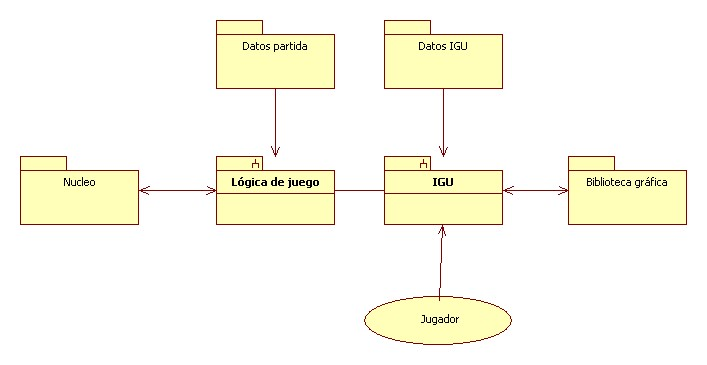
\includegraphics[width=15cm]{images/diagramas/arquitectura.jpg}
	\caption{Diagrama arquitectura}
	\label{fig:Arquitectura}
\end{figure}

\begin{itemize}
	\item \textbf{N�cleo}: Representa los diferentes m�dulos que constituyen en �ltimo t�rmino la l�gica de juego. Estos componentes reciben los datos proporcionados por el jugador y otros m�dulos y procesan en cada turno el siguiente estado de los mismos. El estado de dichos m�dulos es salvable y recuperable.
	\item \textbf{Biblioteca gr�fica}: Proporciona los componentes gr�ficos para el dibujado y la interacci�n con el interfaz de usuario 2D. Tambi�n proporciona mecanismo de control y comunicaci�n entre la parte gr�fica y la l�gica de juego.
	\item \textbf{Datos partida}: En primera instancia estos datos son le�dos de un fichero de configuraci�n XML y definen todas las caracter�sticas iniciales del estado a simular y, por consiguiente, el tipo de partida que el jugador va a experimentar.
	\item \textbf{Datos IGU}: En primera instancia estos datos son le�dos de un fichero de configuraci�n XML y definen todas las caracter�sticas iniciales del interfaz de usuario esto es, su apariencia, posici�n y tipo.
	\item \textbf{L�gica de juego}: Se encarga de controlar el juego sincronizando los diferentes m�dulos. Define cual es el orden de actualizaci�n de los m�dulos y por lo tanto de que manera se genera el siguiente estado en cada turno.
	\item \textbf{IGU}: Captura las entradas del usuario sobre el interfaz de usuario y las transforma de forma que sean elementos significativos para la l�gica de juego.
	\item \textbf{Jugador}: Representa al �nico jugador posible en un momento dado. HONOS es no es juego multijugador, por lo tanto todas las acciones provienen del mismo usuario para una misma partida.
\end{itemize}

\input{dise�o.tex}

\chapter{Implementaci�n}
\label{sec:implementacion}
\section{Est�ndares y normas seguidos}
La implementaci�n del proyecto sigue el est�ndar ISO/IEC   JTC1/SC22/WG21 para C++ en la medida de lo posible, esto es: 
\begin{itemize}
	\item Todo el c�digo escrito espec�ficamente para el proyecto respeta el est�ndar.
	\item No se utiliza ninguna clase/biblioteca de clases de apoyo que no provenga de la estandarizada STL.
	\item En el caso de no cumplirse la segunda condici�n, la clase/ biblioteca de clases utilizada respeta la primera condici�n.
	\item Existe una �nica excepci�n a estas normas en la implementaci�n de ciertos componentes de la biblioteca de clases del interfaz gr�fico de usuario; dicha implementaci�n est� irremediablemente ligada a la tecnolog�a usada para comunicarse con los dispositivos de visualizaci�n, y que en esta implementaci�n concreta, pertenecen a una tecnolog�a propietaria de la que se carece de c�digo fuente, por lo tanto no puede garantizarse la primera condici�n.
\end{itemize}

En cuanto a la construcci�n de las clases, se sigue una pol�tica estricta en cuanto a la inicializaci�n y liberaci�n de recursos, as� como en el tratamiento de errores.

\section{Inicializaci�n y liberaci�n de recursos}
Todos los objetos reservan recursos y se inicializan de forma at�mica en el constructor, aplicando el patr�n de implementaci�n Resource Adquisition Is Initialization (Ver: RAII \ref{sec:raii}). De la misma forma, la destrucci�n de los mismos provoca la liberaci�n incondicional de los recursos.
Los objetos instanciados est�n completamente inicializados y listos para su uso.

\section{Manejo de errores}
Por regla general se evita el uso de excepciones salvo para casos excepcionales, como pueden ser los errores en la inicializaci�n de objetos.

\section{Notaci�n}
Salvo los comentarios, el c�digo est� escrito en ingl�s. Esta decisi�n est� relacionada con la liberaci�n del c�digo del proyecto, esperando que la mayor difusi�n del ingl�s en el �mbito de la programaci�n facilite a quien lo quiera el trabajo con el mismo.\\

En cuanto a la notaci�n para nombrado de clases, m�todos, variables, etc, se ha optado por una variaci�n de la notaci�n h�ngara, simplemente por considerar que facilita la lectura y entendimiento del c�digo. As� pues, la notaci�n es consistente con las siguientes normas:

\begin{table}[H]	
		\begin{tabular}{| l | p{10cm} |}
		\hline
			\textbf{Nombres de clase y estructuras} &	Primera letra en may�scula. Si se compone de dos o m�s palabras no se separan, cada palabra lleva la primera letra en may�scula.\\
			\hline
			\textbf{Nombres de m�todos y funciones} &	Primera letra en min�scula. Si se compone de dos o m�s palabras no se separan, cada palabra lleva la primera letra en may�scula.\\				
			\hline
			\textbf{Booleanos} &	Prefijo b\\
			\hline
			\textbf{Enteros} &	Prefijo i\\
			\hline
			\textbf{Doubles} &	Prefijo d\\
			\hline
			\textbf{Arrays} &	Prefijo a\\
			\hline
			\textbf{Punteros} &	Prefijo p\\
			\hline
			\textbf{Cadenas de caracteres anchos} &	Prefijo ws\\
			\hline
			\textbf{Arrays de caracteres anchos} &	Prefijo pwc\\				
			\hline
			\textbf{Miembros de clase / atributos} &	Prefijo m\\
			\hline
			\textbf{Variables globales} &	Prefijo g\\
			\hline
		\end{tabular}
	\caption{Notaci�n}
	\label{tab:Notaci�n}
\end{table}
\newpage
\input{implementacion/lenguaje.tex}
\newpage
\section{Herramientas y programas}

\subsection{Desarrollo}
Para la implementaci�n del proyecto se ha hecho uso de las siguientes herramientas y programas:

\subsubsection{Entorno de desarrollo}
El proyecto ha sido realizado en la plataforma que ofrece Microsoft en su binomio \emph{Windows XP}, como sistema operativo, y \emph{Visual C++ Express Edition}, como entorno integrado de desarrollo (IDE).\\

Visual C++ Express Edition proporciona un entorno gr�fico de programaci�n para C++. Cuenta con un compilador y un depurador con tecnolog�a propietaria de Microsoft. Es una herramienta destinada a la programaci�n por parte de entusiastas y por lo tanto se trata de una herramienta gratuita. Pese a esto, es lo suficientemente completa y potente como para desarrollar un proyecto de las caracter�sticas de HONOS.

\subsubsection{DirectX}
DirectX es una colecci�n de APIs creadas para facilitar tareas relacionadas con la programaci�n de juegos en la plataforma Microsoft Windows. El kit de desarrollo de DirectX es distribuido gratuitamente por Microsoft. Las bibliotecas de DirectX eran originalmente distribuidas por los desarrolladores de juegos con sus paquetes, pero m�s tarde fueron incluidas en Windows.\\

En este proyecto se hace uso de la API de \emph{Direct3D}, accediendo a ella a trav�s del nuevo framework denominado \emph{DXUT}, que facilita ciertas tareas comunes a la programaci�n de videojuegos como son la inicializaci�n de dispositivos y la captura de eventos generados por los perif�ricos.\\

La versi�n utilizada es DirectX 9.0c, compatible con todos los Sistemas Operativos Windows que soporten 9.0c (RC0).\\

\subsubsection{TinyXML}
TinyXML es una peque�o y muy sencillo parser de XML para C++. Ignora DTDs, el software libre y se distribuyen bajo licencia zlib/libpng (compatible con GPL).\\

La elecci�n de este parser sobre otras alternativas radica en sus propias caracter�sticas: es muy sencillo y muy liviano. Si bien carece de muchas funciones, tiene las suficientes para realizar su trabajo dentro del proyecto. En este caso se ha compilado el c�digo como biblioteca est�tica.


\subsection{Documentaci�n}
Para la redacci�n y procesado de la documentaci�n del proyecto se ha hecho uso de las siguientes herramientas y programas:

\subsubsection{LaTeX y 4Spell}
Para la creaci�n y generaci�n de esta documentaci�n se ha utilizado LaTeX.\\

\emph{LaTeX} es un lenguaje de marcado para documentos, y un sistema de preparaci�n de documentos, formado por un gran conjunto de macros de TeX, escritas inicialmente por Leslie Lamport (LamportTeX) en 1984, con la intenci�n de facilitar el uso del lenguaje de composici�n tipogr�fica creado por Donald Knuth. Es muy utilizado para la composici�n de art�culos acad�micos, tesis y libros t�cnicos, dado que la calidad tipogr�fica de los documentos realizados con LaTeX es comparable a la de una editorial cient�fica de primera l�nea. LaTeX es software libre bajo licencia LPPL.\\

Para la correcci�n ortogr�fica se ha utilizado 4Spell.

\subsubsection{MikTeX}
\emph{MikTeX} se ha utilizado como implementaci�n TeX para Windows.

\subsubsection{TeXnicCenter}
\emph{TeXnicCenter} Se usa como entorno de desarrollo integrado para la realizaci�n de documentos en LaTeX en Windows. TeXnicCenter es software libre bajo licencia GPL.

\subsubsection{StarUML}
\emph{StarUML} es un editor de diagramas UML de c�digo abierto; entre las funciones t�picas permite adem�s obtener diagramas a trav�s de c�digo y generarlo a trav�s de diagramas, aunque el soporte para esto s�lo se da en C++, Java y C\#.

\subsubsection{Doxygen}
Para la generaci�n de documentaci�n detallada del c�digo se ha utilizado \emph{Doxygen}. Doxygen es un Generador de documentaci�n para C++, C, Java, Objective-C, Python, IDL (versiones Corba y Microsoft) y en cierta medida para PHP, C\# y D. Dado que es f�cilmente adaptable, funciona en la mayor�a de sistemas Unix as� como en Windows y Mac OS X. La mayor parte del c�digo de Doxygen est� escrita por Dimitri van Heesch.\\

Doxygen es un acr�nimo de dox(document) gen(generator), generador de documentaci�n para c�digo fuente.

\subsubsection{Zotero}
Para la recopilaci�n de bibliograf�a se ha hecho un uso intensivo del programa \emph{Zotero} exportando los resultados a BibTeX (una herramienta para dar formato a listas de referencias que se utiliza habitualmente con el sistema de preparaci�n de documentos LaTeX).\\

Zotero es una extensi�n libre para el navegador Firefox, que permite a los usuarios recolectar, administrar y citar investigaciones de todo tipo de or�genes del navegador. Es parcialmente una aplicaci�n de administraci�n de referencias, usada para administrar bibliograf�as y referencias al escribir ensayos y art�culos.
\newpage
\section{Descripci�n de los ficheros de configuraci�n}
A continuaci�n se decriben los formatos de los ficheros XML que corresponden a la configuraci�n de los diferentes elementos del juego.\\

Junto a ellos aparecen tablas explicativas con el significado de los elementos, atributos y valores.\\

%\subsection{Configuraci�n de los par�metros del pa�s}
%En este fichero se describen los par�metros generales que rigen el pa�s. Mediante la edici�n del mismo se puede dar lugar a diferentes estados a fin de simular realidades sociales diferentes.\\
%\lstset{% general command to set parameter(s)
%language=XML,
%basicstyle=\small, % print whole listing small
%keywordstyle=\color{black}\bfseries,
%stringstyle=\ttfamily, % typewriter type for strings
%showstringspaces=false} % no special string spaces
%\begin{lstlisting}
%<?xml version="1.0" ?>
%<GUI>
%	<Office winter="" fall="" spring="" summer="">
%		<Desk x="" y="" file="">
%			<telephone x="" y="" file=""/>
%			<papers x="" y="" file=""/>
%			<computer x="" y="" file=""/>
%		</Desk>
%		<door x="" y="" file=""/>
%		<balcony x="" y="" file=""/>
%		<eventTab x="" y="" file=""/>
%		<diplomacyButton x="" y="" file="" pressedFile=""/>
%		<countryButton x="" y="" file="" pressedFile=""/>
%		<policiesButton x="" y="" file="" pressedFile=""/>
%		<turnButton x="" y="" file=""  pressedFile=""/>
%		<menuButton x="" y="" file="" pressedFile=""/>
%		<dateArea x="" y="" file=""/>
%	</Office>
%</GUI>
%\end{lstlisting}
%
%\begin{table}[H]
%\begin{tabular}{ | l | l | p{10cm} |}
%\hline
%\textbf{Elemento} & \textbf{Descripci�n} & \textbf{Rango} \\
%\hline
%col 1 & Duraci�n de la partida & La partida tendr� una duraci�n m�nima igual al n�mero de turnos de una legislatura. Al final de esta se aplica la condici�n de �xito para determinar la continuidad\\
%\hline
%\end{tabular}
%\caption{Configuraci�n de los par�metros del pa�s}
%\end{table}

\subsection{Configuraci�n del interfaz de usuario}
De este archivo se obtiene la configuraci�n de los elementos que conforman el interfaz de usuario as� como los recursos (texto y gr�ficos) que necesitan.\\
\lstset{% general command to set parameter(s)
language=XML,
basicstyle=\small, % print whole listing small
keywordstyle=\color{black}\bfseries,
stringstyle=\ttfamily, % typewriter type for strings
showstringspaces=false} % no special string spaces
\begin{lstlisting}
<?xml version="1.0" ?>

<uicomponent type="image" id="background"  x="0" y="0" z="0"  texture1="resources/images/despachoNew.png"/>

<uicomponent type="button" id="openTelephone"  x="60" y="324" z="1"  texture1="resources/images/diplomacyButton.png" texture2="resources/images/diplomacyButton.png"/>
<uicomponent type="button" id="openPolitics"  x="904" y="324" z="1"  texture1="resources/images/politicsButton.png" texture2="resources/images/politicsButton.png"/>
<uicomponent type="button" id="openComputer"  x="512" y="648" z="1"  texture1="resources/images/computerButton.png" texture2="resources/images/computerButton.png"/>

<uicomponent type="image" id="telephone"  x="0" y="112" z="2"  texture1="resources/images/telephone.png"/>
<uicomponent type="textArea" id="chatingLabel"  x="0" y="115" z="2" w="60" h="20"  text="Al telefono: "/>
<uicomponent type="textArea" id="chatingValue"  x="60" y="115" z="2" w="60" h="20"  text=""/>
<uicomponent type="image" id="franceButton"  x="264" y="274" z="2" w="20" h="20" />
<uicomponent type="image" id="englandButton"  x="360" y="285" z="2" w="20" h="20"/>
<uicomponent type="image" id="usaButton"  x="300" y="315" z="2" w="20" h="20" />
<uicomponent type="button" id="nextTreatyButton"  x="20" y="350" z="2" texture1="resources/images/nextUp.png" texture2="resources/images/nextDown.png"/>
<uicomponent type="button" id="signTreatyButton"  x="220" y="350" z="2" texture1="resources/images/squareButton.png" texture2="resources/images/squareButton.png"/>
<uicomponent type="textArea" id="activeTreaty"  x="10" y="350" z="2" w="10" h="20" text=""/>
<uicomponent type="textArea" id="treatyName"  x="100" y="350" z="2" w="250" h="20"  text="Nombre tratado"/>
<uicomponent type="image" id="signedTreatyImage"  x="350" y="370" z="2"  texture1="resources/images/signedPolicy.png"/>

<uicomponent type="image" id="computer"  x="256" y="468" z="1"  texture1="resources/images/computer.png"/>

<uicomponent type="image" id="production"  x="296" y="490" z="2"  texture1="resources/images/foo.png"/>

<uicomponent type="textArea" id="foodLabel"  x="356" y="520" z="2" w="137" h="20"  text="Alimentacion"/>
<uicomponent type="textArea" id="foodStatusLabel"  x="356" y="540" z="2" w="137" h="20"  text="Estado de la produccion: "/>
<uicomponent type="textArea" id="foodStatusValue"  x="493" y="540" z="2" w="137" h="20"  text=""/>
<uicomponent type="textArea" id="foodConsuptionLabel"  x="356" y="560" z="2" w="58" h="20"  text="Consumo: "/>
<uicomponent type="textArea" id="foodConsuptionValue"  x="493" y="560" z="2" w="58" h="20"  text=""/>
<uicomponent type="slider" id="foodTaxSlider"  x="554" y="530" z="2"  texture1="resources/images/sliderBar.png" texture2="resources/images/sliderButton.png"/>
<uicomponent type="textArea" id="foodTaxSliderLabel"  x="590" y="515" z="2" w="58" h="20"  text="Impuestos: "/>
<uicomponent type="textArea" id="foodTaxSliderValue"  x="650" y="515" z="2" w="58" h="20"  text="0%"/>
<uicomponent type="textArea" id="foodSubventionLabel"  x="590" y="555" z="2" w="58" h="20"  text="Subvencion: "/>
<uicomponent type="textArea" id="foodSubventionValue"  x="650" y="555" z="2" w="58" h="20"  text="0%"/>
<uicomponent type="slider" id="foodSubventionSlider"  x="554" y="570" z="2"  texture1="resources/images/sliderBar.png" texture2="resources/images/sliderButton.png"/>

<uicomponent type="textArea" id="energyLabel"  x="356" y="612" z="2" w="137" h="20"  text="Energia"/>
<uicomponent type="textArea" id="energyStatusLabel"  x="356" y="632" z="2" w="137" h="20"  text="Estado de la produccion: "/>
<uicomponent type="textArea" id="energyStatusValue"  x="493" y="632" z="2" w="137" h="20"  text=""/>
<uicomponent type="textArea" id="energyConsuptionLabel"  x="356" y="652" z="2" w="58" h="20"  text="Consumo: "/>
<uicomponent type="textArea" id="energyConsuptionValue"  x="493" y="652" z="2" w="58" h="20"  text=""/>
<uicomponent type="textArea" id="energyTaxSliderLabel"  x="590" y="607" z="2" w="58" h="20"  text="Impuestos: "/>
<uicomponent type="textArea" id="energyTaxSliderValue"  x="650" y="607" z="2" w="58" h="20"  text="0%"/>
<uicomponent type="slider" id="energyTaxSlider"  x="554" y="622" z="2"  texture1="resources/images/sliderBar.png" texture2="resources/images/sliderButton.png"/>
<uicomponent type="textArea" id="energySubventionLabel"  x="590" y="647" z="2" w="58" h="20"  text="Subvencion: "/>
<uicomponent type="textArea" id="energySubventionValue"  x="650" y="647" z="2" w="58" h="20"  text="0%"/>
<uicomponent type="slider" id="energySubventionSlider"  x="554" y="662" z="2"  texture1="resources/images/sliderBar.png" texture2="resources/images/sliderButton.png"/>

<uicomponent type="textArea" id="manufacturedLabel"  x="356" y="699" z="2" w="137" h="20"  text="Pro. manufacturados"/>
<uicomponent type="textArea" id="manufacturedStatusLabel"  x="356" y="719" z="2" w="137" h="20"  text="Estado de la produccion: "/>
<uicomponent type="textArea" id="manufacturedStatusValue"  x="493" y="719" z="2" w="137" h="20"  text=""/>
<uicomponent type="textArea" id="manufacturedConsuptionLabel"  x="356" y="739" z="2" w="58" h="20"  text="Consumo: "/>
<uicomponent type="textArea" id="manufacturedConsuptionValue"  x="493" y="739" z="2" w="58" h="20"  text=""/>
<uicomponent type="textArea" id="manufacturedTaxSliderLabel"  x="590" y="694" z="2" w="58" h="20"  text="Impuestos: "/>
<uicomponent type="textArea" id="manufacturedTaxSliderValue"  x="650" y="694" z="2" w="58" h="20"  text="0%"/>
<uicomponent type="slider" id="manufacturedTaxSlider"  x="554" y="709" z="2"  texture1="resources/images/sliderBar.png" texture2="resources/images/sliderButton.png"/>
<uicomponent type="textArea" id="manufacturedSubventionLabel"  x="590" y="731" z="2" w="58" h="20"  text="Subvencion: "/>
<uicomponent type="textArea" id="manufacturedSubventionValue"  x="650" y="731" z="2" w="58" h="20"  text="0%"/>
<uicomponent type="slider" id="manufacturedSubventionSlider"  x="554" y="746" z="2"  texture1="resources/images/sliderBar.png" texture2="resources/images/sliderButton.png"/>

<uicomponent type="image" id="ssss"  x="296" y="490" z="3"  texture1="resources/images/foo2.png"/>
<uicomponent type="textArea" id="healthLabel"  x="356" y="520" z="2" w="137" h="20"  text="Sanidad"/>
<uicomponent type="textArea" id="healthStatusLabel"  x="356" y="540" z="2" w="137" h="20"  text="Estado del servicio: "/>
<uicomponent type="textArea" id="healthStatusValue"  x="493" y="540" z="2" w="137" h="20"  text=""/>
<uicomponent type="textArea" id="healthCostLabel"  x="356" y="560" z="2" w="58" h="20"  text="Coste: "/>
<uicomponent type="textArea" id="healthCostValue"  x="493" y="560" z="2" w="58" h="20"  text=""/>
<uicomponent type="slider" id="healthSalarySlider"  x="554" y="530" z="3"  texture1="resources/images/sliderBar.png" texture2="resources/images/sliderButton.png"/>
<uicomponent type="textArea" id="healthSalarySliderLabel"  x="590" y="515" z="2" w="58" h="20"  text="Salario: "/>
<uicomponent type="textArea" id="healthSalarySliderValue"  x="650" y="515" z="2" w="58" h="20"  text="0%"/>
<uicomponent type="textArea" id="healthSubventionLabel"  x="590" y="555" z="2" w="58" h="20"  text="Recursos: "/>
<uicomponent type="textArea" id="healthSubventionValue"  x="650" y="555" z="2" w="58" h="20"  text="0%"/>
<uicomponent type="slider" id="healthCostSlider"  x="554" y="570" z="3"  texture1="resources/images/sliderBar.png" texture2="resources/images/sliderButton.png"/>

<uicomponent type="textArea" id="educationLabel"  x="356" y="612" z="2" w="137" h="20"  text="Educacion"/>
<uicomponent type="textArea" id="educationStatusLabel"  x="356" y="632" z="2" w="137" h="20"  text="Estado del servicio: "/>
<uicomponent type="textArea" id="educationStatusValue"  x="493" y="632" z="2" w="137" h="20"  text=""/>
<uicomponent type="textArea" id="educationCostLabel"  x="356" y="652" z="2" w="58" h="20"  text="Coste: "/>
<uicomponent type="textArea" id="educationCostValue"  x="493" y="652" z="2" w="58" h="20"  text=""/>
<uicomponent type="slider" id="educationSalarySlider"  x="554" y="622" z="3"  texture1="resources/images/sliderBar.png" texture2="resources/images/sliderButton.png"/>
<uicomponent type="textArea" id="educationSalarySliderLabel"  x="590" y="607" z="2" w="58" h="20"  text="Salario: "/>
<uicomponent type="textArea" id="educationSalarySliderValue"  x="650" y="607" z="2" w="58" h="20"  text="0%"/>
<uicomponent type="textArea" id="educationSubventionLabel"  x="590" y="647" z="2" w="58" h="20"  text="Recursos: "/>
<uicomponent type="textArea" id="educationSubventionValue"  x="650" y="647" z="2" w="58" h="20"  text="0%"/>
<uicomponent type="slider" id="educationCostSlider"  x="554" y="662" z="3"  texture1="resources/images/sliderBar.png" texture2="resources/images/sliderButton.png"/>

<uicomponent type="textArea" id="justiceLabel"  x="356" y="699" z="2" w="137" h="20"  text="Justicia"/>
<uicomponent type="textArea" id="justiceStatusLabel"  x="356" y="719" z="2" w="137" h="20"  text="Estado del servicio: "/>
<uicomponent type="textArea" id="justiceStatusValue"  x="493" y="719" z="2" w="137" h="20"  text=""/>
<uicomponent type="textArea" id="justiceCostLabel"  x="356" y="739" z="2" w="58" h="20"  text="Coste: "/>
<uicomponent type="textArea" id="justiceCostValue"  x="493" y="739" z="2" w="58" h="20"  text=""/>
<uicomponent type="slider" id="justiceSalarySlider"  x="554" y="709" z="3"  texture1="resources/images/sliderBar.png" texture2="resources/images/sliderButton.png"/>
<uicomponent type="textArea" id="justiceSalarySliderLabel"  x="590" y="694" z="2" w="58" h="20"  text="Salario: "/>
<uicomponent type="textArea" id="justiceSalarySliderValue"  x="650" y="694" z="2" w="58" h="20"  text="0%"/>
<uicomponent type="textArea" id="justiceSubventionLabel"  x="590" y="731" z="2" w="58" h="20"  text="Recursos: "/>
<uicomponent type="textArea" id="justiceSubventionValue"  x="650" y="731" z="2" w="58" h="20"  text="0%"/>
<uicomponent type="slider" id="justiceCostSlider"  x="554" y="746" z="3"  texture1="resources/images/sliderBar.png" texture2="resources/images/sliderButton.png"/>


<uicomponent type="image" id="productionTab"  x="643" y="474" z="2"  texture1="resources/images/footab.png"/>
<uicomponent type="image" id="ssssTab"  x="573" y="474" z="3"  texture1="resources/images/foo2tab.png"/>


<uicomponent type="image" id="politics"  x="579" y="112" z="2"  texture1="resources/images/politics.png"/>

<uicomponent type="button" id="closeTelephone"  x="429" y="112" z="2"  texture1="resources/images/closeButton.png" texture2="resources/images/closeButton.png"/>
<uicomponent type="button" id="closePolitics"  x="579" y="112" z="2"  texture1="resources/images/closeButton.png" texture2="resources/images/closeButton.png"/>
<uicomponent type="button" id="closeComputer"  x="742" y="468" z="2"  texture1="resources/images/closeButton.png" texture2="resources/images/closeButton.png"/>\end{lstlisting}

\begin{table}[H]
\begin{tabular}{ | l | p{8cm} | l |}
\hline
\textbf{Elemento} & \textbf{Descripci�n} & \textbf{Rango} \\
\hline
\emph{uicomponent} & Representa un componente de la interfaz de usuario & -\\
\hline
\emph{type} & Tipo de componente de la interfaz de usuario & image, button, slider o textArea\\
\hline
\emph{id} & Identificador �nico del componente & -\\
\hline
\emph{x} & Posic�n horizontal del componente en pixels & [0,1024]\\
\hline
\emph{y} & Posic�n vertical del componente en pixels & [0,768]\\
\hline
\emph{z} & Profundidad del componente & [0,4]\\
\hline
\emph{w} & Ancho en pixels del componente & [0,1024]\\
\hline
\emph{h} & Largo en pixels del componente & [0,768]\\
\hline
\emph{texture1} & Ruta a la imagen que sirve de textura principal (buttons, sliders, images y textAreas) o barra de desplazamiento (sliders) & - \\
\hline
\emph{texture2} & Ruta a la imagen que sirve de textura secundaria (buttons) o bot�n de desplazamiento (sliders) & - \\
\hline
\emph{text} & Texto del componente (button y textArea) & - \\
\hline
\end{tabular}
\caption{Configuraci�n del interfaz de usuario}
\end{table}

\subsection{Configuraci�n de actividades pol�ticas}
En este archivo se definen todas las actividades pol�ticas (internas o diplom�ticas) disponibles a lo largo del juego.
\lstset{% general command to set parameter(s)
language=XML,
basicstyle=\small, % print whole listing small
keywordstyle=\color{black}\bfseries,
stringstyle=\ttfamily, % typewriter type for strings
showstringspaces=false} % no special string spaces
\begin{lstlisting}
<?xml version="1.0" ?>

<treatyList>

<treaty country="france" name="Tratado comercial" description="Este tratado supone jugosas ventajas comerciales.">
	<requeriment type="ss_healthcare_personal" value="0" interval="1"/>	
	<requeriment type="pr_energy_np" value="0" interval="1"/>	
	<effect type=pr_all_cp" value="-0.5"/>
	<effect type="pr_energy_ni" value="0.1"/>
</treaty>

<treaty country="france" name="Ejemplo de tratado" description="Descripci�n del tratado">
	<requeriment type="ss_all_salary" value="0.5" interval="0"/>	
	<effect type="ss_healthcare_personal" value="0.06"/>
</treaty>

<treaty country="france" name="Ejemplo de tratado 2" description="Descripci�n del tratado 2">
	<requeriment type="ss_all_salary" value="0.5" interval="0"/>	
	<effect type="ss_healthcare_personal" value="0.06"/>
</treaty>
</treatyList>
\end{lstlisting}

\begin{table}[H]
\begin{tabular}{ | l | p{8cm} | l |}
\hline
\textbf{Elemento} & \textbf{Descripci�n} & \textbf{Rango} \\
\hline
\emph{treaty} & Tratado diplom�tico & -\\
\hline
\emph{country} & Destinatario del tratado diplom�tico & france, england o usa\\
\hline
\emph{name} & Nombre del tratado & -\\
\hline
\emph{description} & Descripci�n del tratado & -\\
\hline
\emph{requeriment} & Describe un requerimiento de una actividad pol�tica & -\\
\hline
\emph{effect} & Describe un efecto de una actividad pol�tica & -\\
\hline
\emph{type} & Indica a que factor de la simulaci�n afecta & -\\
\hline
\emph{value} & Indica el valor necesario para cumplir el requerimiento (requeriment) o el bonus del efecto (effect) & -\\
\hline
\emph{interval} & Indica el intervalo en que puede variar un requerimiento para seguir siendo cumplido & -\\
\hline
\end{tabular}
\caption{Configuraci�n de las actividades pol�ticas}
\end{table}

\subsection{Configuraci�n de grupos de poblaci�n}
En este archivo se guarda la configuraci�n de los diferentes grupos poblacionales. Mediante su edici�n podemos conformar sociedades m�s o menos heterogeneas.\\
\lstset{% general command to set parameter(s)
language=XML,
basicstyle=\small, % print whole listing small
keywordstyle=\color{black}\bfseries,
stringstyle=\ttfamily, % typewriter type for strings
showstringspaces=false} % no special string spaces
\begin{lstlisting}
<?xml version="1.0" ?>
<population>
	
	<populationGroup name="conservatives" size="0.2" purchasingPower="0.2">
		<opinion type="health">0.5</opinion>
		<opinion type="food">1</opinion>
		<opinion type="energy">1</opinion>
		<opinion type="manufactured">1</opinion>
		<opinion type="education">1</opinion>
		<opinion type="justice">1</opinion>
	</populationGroup>
	
	<populationGroup name="merchants" size="0.2" purchasingPower="0.2">
		<opinion type="health">0.5</opinion>
		<opinion type="food">1</opinion>
		<opinion type="energy">1</opinion>
		<opinion type="manufactured">1</opinion>
		<opinion type="education">1</opinion>
		<opinion type="justice">1</opinion>
	</populationGroup>
	
	<populationGroup name="ultrademocrats" size="0.2" purchasingPower="0.2">
		<opinion type="health">0.6</opinion>
		<opinion type="food">2</opinion>
		<opinion type="energy">1</opinion>
		<opinion type="manufactured">1</opinion>
		<opinion type="education">1</opinion>
		<opinion type="justice">1</opinion>
	</populationGroup>
	
	<populationGroup name="asilanders" size="0.2" purchasingPower="0.2">
		<opinion type="health">0.5</opinion>
		<opinion type="food">1</opinion>
		<opinion type="energy">1</opinion>
		<opinion type="manufactured">1</opinion>
		<opinion type="education">1</opinion>
		<opinion type="justice">1</opinion>
	</populationGroup>
	
	<populationGroup name="greens" size="0.2" purchasingPower="0.2">
		<opinion type="health">0.5</opinion>
		<opinion type="food">1</opinion>
		<opinion type="energy">1</opinion>
		<opinion type="manufactured">1</opinion>
		<opinion type="education">1</opinion>
		<opinion type="justice">1</opinion>
	</populationGroup>
	
</population>
\end{lstlisting}

\begin{table}[H]
\begin{tabular}{ | l | p{8cm} | p{3cm} |}
\hline
\textbf{Elemento} & \textbf{Descripci�n} & \textbf{Rango} \\
\hline
\emph{populationGroup} & Representa un grupo de poblaci�n & -\\
\hline
\emph{name} & Nombre del grupo de poblaci�n & conservatives, merchants, aislanders, greens o ultrademocrats\\
\hline
\emph{size} & Porcentaje de poblaci�n que representa el grupo & [0,1]\\
\hline
\emph{purchansingPower} & Porcentaje de riqueza que acumula el grupo & [0,1]\\
\hline
\emph{opinion} & Representa una opini�n sobre cierto par�metro del pa�s & [0,1]\\
\hline
\emph{type} & Indica a que factor de la simulaci�n la que afecta &  health, food, manufactured, education o justice\\
\hline
\end{tabular}
\caption{Configuraci�n de los grupos de poblaci�n}
\end{table}

\subsection{Configuraci�n de productos}
En este archivo se describen las caracter�sticas de cada uno de los productos que conforman la producci�n del estado del jugador.\\
\lstset{% general command to set parameter(s)
language=XML,
basicstyle=\small, % print whole listing small
keywordstyle=\color{black}\bfseries,
stringstyle=\ttfamily, % typewriter type for strings
showstringspaces=false} % no special string spaces
\begin{lstlisting}
<?xml version="1.0" ?>
<production>
	<product name="food" np="1.0" cp="1.0"  maxStorageCapacity="10" maxTotalProduct="5.0" money="10.0" storage="10"/>
	<product name="energy" np="1.0" cp="1.0"  maxStorageCapacity="10" maxTotalProduct="5.0" money="10.0" storage="10"/>
	<product name="manufactured" np="1.0" cp="1.0"  maxStorageCapacity="10" maxTotalProduct="5.0" money="10.0" storage="10"/>
</production>
\end{lstlisting}

\begin{table}[H]
\begin{tabular}{ | l | p{5cm} | l |}
\hline
\textbf{Elemento} & \textbf{Descripci�n} & \textbf{Rango} \\
\hline
\emph{product} & Representa un producto de la producci�n & -\\
\hline
\emph{name} & Nombre del producto de la producci�n & food, energy o manufactured\\
\hline
\emph{np} & N�mero de unidades que inicial produciendo & > 0\\
\hline
\emph{np} & Coste de producci�n por unidad & > 0\\
\hline
\emph{maxStorageCapacity} & M�xima capacidad de almacenaje de unidades & > 0\\
\hline
\emph{maxTotalProduct} & M�xima capacidad de almacenaje de producci�n & > 0\\
\hline
\emph{money} & Dinero disponible inicialmente & > 0\\
\hline
\emph{storage} & Almacen disponible inicialmente & > 0\\
\hline
\end{tabular}
\caption{Configuraci�n de los productos}
\end{table}

\subsection{Configuraci�n de los servicios sociales}
En este archivo se describen las caracter�sticas de cada uno de los servicios sociales del estado del jugador.\\

\lstset{% general command to set parameter(s)
language=XML,
basicstyle=\small, % print whole listing small
keywordstyle=\color{black}\bfseries,
stringstyle=\ttfamily, % typewriter type for strings
showstringspaces=false} % no special string spaces
\begin{lstlisting}
<?xml version="1.0" ?>
<socialServices>
	<socialService name="health" salaryop="1000.0" resourcesop="2000.0" personalImportance="0.5" resourcesImportance="0.5"/>
	<socialService name="education" salaryop="1000.0" resourcesop="2000.0" personalImportance="0.5" resourcesImportance="0.5"/>
	<socialService name="justice" salaryop="1000.0" resourcesop="2000.0" personalImportance="0.5" resourcesImportance="0.5"/>
</socialServices>\end{lstlisting}

\begin{table}[H]
\begin{tabular}{ | l | p{5cm} | p{5cm} |}
\hline
\emph{socialService} & Representa un servicio social & -\\
\hline
\emph{name} & Nombre del servicio social & health, education o justice\\
\hline
\emph{salaryop} & Salario �ptimo para el personal & > 0\\
\hline
\emph{resourcesop} & Inversi�n �ptima en recursos materiales & > 0\\
\hline
\emph{personalImportance} & Importancia del personal & [0,1] \\
\hline
\emph{resources Importance} & Importancia de los recursos materiales & [0,1] \\
\hline
\end{tabular}
\caption{Configuraci�n de los servicios sociales}
\end{table}
%\input{implementacion/descripcion-clases.tex}


%\input{memoria.tex}
%
%\input{metodologia.tex}
%
%\input{conclusiones.tex}
%
%\appendix
%
\chapter{Manual de Usuario}
\label{sec:manual}

\section{HONOS}
\emph{HONOS} es un juego de tipo simulador donde el asumir�s el papel de jefe de estado de un pa�s imaginario. Reci�n electo como presidente, dispondr�s de 4 a�os para acometer las pol�ticas que considere oportunas con miras a que tu pa�s evolucione favorablemente y, porque no, a la reelecci�n.

En HONOS tendr�s que gestionar los recursos de tu pa�s, definir tu relaci�n con otros estados, tomar decisiones sobre importantes eventos as� como promover y ejecutar pol�ticas que definan el rumbo de tu pa�s. �Qui�n decidir� si estas haciendo un buen trabajo? Ser� el pueblo quien juzgue tus acciones, pero recuerda, la poblaci�n es una masa heterog�nea con intereses y posturas diferentes.

\section{La historia pol�tica de Prunisia}

Prunisia:

\begin{itemize}
	\item Extensi�n: 115.300 km2
	\item N� de habitantes:
\end{itemize}

Entre los a�os 450 y 430adC diversas expediciones atenienses arriban en la isla situada a 40 millas al suroeste de las islas brit�nicas, que posteriormente bautizar�an como Prunisia, y pronto se establecen de forma permanente. En principio el destino de Prunisia iba a ser el de parada intermedia de las aventuras mar�timas griegas en el norte de Europa. Sin embargo, las dificultades que supon�a cada viaje y la lejan�a con la polis griega pronto hacen desistir de esta empresa. Los escasos abor�genes (se cree que de origen celta) no son capaces de oponer demasiada resistencia contra las bien preparadas tropas griegas y pronto son absorbidos por la incipiente polis griega de Prunisia.\\

Pronto empiezan aparecer claras diferencias en la sociedad pruna que se manifiestan en las disputas concernientes a las relacionas con el continente. Los partidarios de una relaci�n abierta que basada fundamentalmente en el comercio, medran a un ritmo vertiginoso comparado con su m�s recelosos vecinos. Este aumento de capital acrecienta m�s si cabe las diferencias entre hombres libres y esclavos, pero adem�s abre nuevas brechas inexistentes hasta entonces entre los hombres libres.\\
%Tiene que haber una forma m�s f�cil de hacer esto..
\newcounter{siglo} 
\setcounter{siglo}{16}
Poco a poco, los ciudadanos m�s pudientes alcanzan un mayor poder de representaci�n que se traduce tras siglos de avance, a mediados del \Roman{siglo}, en la creaci�n de un sistema de castas definido desde el nacimiento del que es ya casi imposible escapar. Hasta los m�s recelosos han abierto sus brazos al comercio exterior pero ninguna fortuna, por grande que fuese, era capaz de comprar tanto poder como el que ostentaban los arist�cratas, aunados bajo la figura del emperador y due�os de un, aunque poco numeroso, bien entrenado ej�rcito profesional, el poder real es ejercido por una minor�a de los prunos.\\
\setcounter{siglo}{19}
Sin embargo, las semillas democr�ticas depositadas por los griegos estaban demasiado enraizadas para ser completamente olvidadas. La tradici�n protodemocr�tica y las ideas de la Ilustraci�n que se cuelan en la isla, son el germen de una Revoluci�n con grandes similitudes a la francesa, pero ya en pleno siglo \Roman{siglo}.\\

Hasta nuestros d�as el poder pol�tico se ha ido alternando entre distintas facciones, y aunque los primeros d�as de verdadera democracia se acometieron grandes cambios, diversos, y m�s o menos desastrosos gobiernos, han ido mermando la fe del pueblo en la clase pol�tica dirigente.
Ahora es tu turno\ldots \\

Eres el reci�n electo presidente de Prunisia. El m�s joven en toda la historia de la democracia pruna. Tienes 4 a�os para demostrar que los que buscaban un cambio apostando por sangre joven acertaron. �Pasar�s a la historia como el m�s revolucionario presidente o como el m�s desastroso? 
\begin{quote}
	\emph{A fructibus cognoscitur arbor}\\
	(A un �rbol se lo conoce por sus frutos)
\end{quote}

\section{�C�mo jugar? Inicio r�pido}

\subsection{Inicio}
En la pantalla principal selecciona Nueva Partida, introduce tu nombre y pulsa Comenzar. A continuaci�n aparecer� la pantalla de bienvenida y despu�s la pantalla Despacho.\\
                                         (Imagen:Pantalla de bienvenida) (Imagen: Pantalla despacho)
                                         
\begin{itemize}
	\item Click en el ordenador o pulsa bot�n O para acceder a la pantalla Ordenador. Desde ella puedes acceder a la informaci�n sobre la situaci�n actual de tu pa�s, as� como intervenir en el desarrollo de la producci�n y el funcionamiento de los servicios p�blicos.
	\item Click en los papeles sobre el escritorio o pulsa bot�n P para acceder a la pantalla Pol�ticas. Desde ella puedes revisar las pol�ticas disponibles y seleccionar cuales deseas que se lleven a cabo.
	\item Click en el tel�fono o pulsa el bot�n I para acceder a la pantalla Relaciones internacionales. Desde ella puedes seleccionar el embajador con el que quieres hablar para establecer relaciones internacionales.
	\item Click en la puerta o pulsa el bot�n ESC para acceder a la pantalla de Opciones. Desde ella puedes acceder a las opciones de guardado, carga y fin de juego. 
\end{itemize}


\subsection{Turnos}
El desarrollo del juego se lleva a cabo a trav�s de turnos. En cada uno de ellos se puedes estudiar la situaci�n del pa�s, tomar decisiones en forma de pol�ticas, tratar de establecer relaciones internacionales, etc. Las medidas adoptadas se llevar�n a cabo al avanzar al siguiente turno.\\

                                              (Imagen: Contador de turnos)

En la esquina inferior derecha aparece el contador de turnos, indicando el turno actual y los turnos restantes para finalizar la legislatura. Cuando quieras avanzar al siguiente turno haz click con el rat�n en el bot�n situado a la derecha o bien pulsa la tecla t.\\

\subsection{Atender eventos}
Si el indicador de eventos est� encendido no podr�s avanzar turno hasta que lo atiendas. Click con el rat�n sobre el o pulsa el bot�n U para acceder la pantalla de eventos.

\section{Pantalla de juego}

\subsection{Despacho}
La pantalla principal del juego representa tu despacho. Hay diferentes elementos con los que puedes interactuar para llevar a cabo tus tareas, haciendo click sobre los elementos:

                                              (Imagen: Despacho)

\begin{itemize}
	\item Pol�ticas: Abre la ventana con el interfaz de pol�ticas. Las pol�ticas te permiten tomar decisiones respecto a como orientar la pol�tica en tu mandato.
	\item Ordenador: Abre la ventana con el interfaz del ordenador. El ordenador te servir� para recopilar informaci�n sobre el estado de tu pa�s y su poblaci�n. Tambi�n te permitir� administrar los recursos y servicios.
	\item Puerta: Despliega el men� de opciones.
	\item Tel�fono: Abre el men� de relaciones internacionales. Las relaciones internacionales definen tu relaci�n con potencias extranjeras.
	\item Turno: Muestra el turno actual, los turno que restan para finalizar la legislatura y permite avanzar al siguiente turno.
	\item Aviso de evento: Este indicador se ilumina siempre que exista alg�n evento que requiera atenci�n inmediata. 
\end{itemize}  

A excepci�n del men� de opciones, es posible tener en pantalla diferentes interfaces. Por ejemplo, abrimos la ventana de Pol�ticas para seleccionar alguna nueva medida que queremos implementar, al mismo tiempo podemos abrir la ventana del ordenador para comprobar datos que nos ayuden a tomar una decisi�n.\\

\subsection{Informe de pol�ticas}
Desde esta pantalla puedes navegar por las pol�ticas que est�n disponibles para aplicar en este momento. La informaci�n indica, adem�s de una descripci�n textual un breve resumen que tus asesores elaboran para se�alar los efectos aproximados que la aplicaci�n de la pol�tica tendr� en la poblaci�n, as� como el gasto que supondr� su implantaci�n.\\

                                              (Imagen: Informe pol�ticas)
\begin{itemize}
	\item Men� con las diferentes categor�as de pol�ticas. Al pulsar '+' se despliegan las pol�ticas disponibles de la categor�a.
	\item Pol�tica seleccionada.
	\item T�tulo pol�tica seleccionada.
	\item Descripci�n de la pol�tica.
	\item Descripci�n de los efectos y gastos.
	\item Aprueba la ley. 
\end{itemize} 

\subsection{Ordenador}
El ordenador te permite acceder a gran cantidad de informaci�n relevante sobre el estado de tu pa�s. Desde aqu� puedes acceder a las encuestas de popularidad que indican el nivel actual de satisfacci�n de las diferentes clases sociales, tambi�n puedes acceder a informaci�n sobre el estado de la producci�n y de los servicios sociales.

                                              (Imagen: Informe ordenador)

Adem�s de revisar datos, puedes intervenir variando ciertos par�metros, como se explicar� a continuaci�n. Seleccionar el icono correspondiente a las estad�sticas (Imagen: icono estad�sticas) o pulsar el bot�n E abre la pantalla Estad�sticas. Aqu� aparece informaci�n del estado actual de tu popularidad con respecto a cada clase social; adem�s el gr�fico muestra la evoluci�n, desde el inicio de la legislatura hasta el turno actual, de tu popularidad. Para obtener m�s informaci�n sobre las clases sociales y la poblaci�n en general, consultar La poblaci�n.\\

                                              (Imagen: Estad�sticas)

Seleccionar el icono de producci�n (Imagen: icono producci�n) o pulsar la tecla R abre el interfaz para la gesti�n de recursos. Cada pesta�a representa un recurso; sobre �l se muestra informaci�n (nombre, descripci�n, precio, producci�n actual, reservas, cantidad de importaci�n/exportaci�n); otra parte del interfaz permite variar la unidades producidas por turno, las destinadas a la importaci�n y la exportaci�n. Para m�s informaci�n sobre que significa cada elemento, que supone la varianza de la producci�n y en general cualquier informaci�n m�s detallada, consultar Los recursos.\\

                                              (Imagen: Producci�n)
\begin{itemize}
	\item Recursos.
	\item Nombre y descripci�n del producto seleccionado.
	\item Informaci�n sobre la producci�n (unidades producidas por turno, precio, reservas, cantidad de importaci�n/exportaci�n)
	\item 
	\item Aceptar los cambios realizados.
	\item Cancelar los cambios realizados. 
\end{itemize}  

Seleccionar el icono de servicios sociales (Imagen: icono servicios sociales) o pulsar la tecla T abre la pantalla de servicios sociales. Cada pesta�a representa uno de los grupos de servicios que ofrece el estado (justicia, sanidad y defensa); sobre �l se muestra informaci�n (nombre, descripci�n, nivel de calidad, personal asignado, gasto por turno); otra parte del interfaz permite variar ciertos par�metros como son el personal asignado o la inversi�n en el servicio en cuesti�n. Para m�s informaci�n sobre que significa cada elemento, que supone la varianza de la inversi�n y en general cualquier informaci�n m�s detallada, consultar Infraestructuras y servicios.

                                              (Imagen: Servicios)

\begin{itemize}
	\item Servicios.
	\item Nombre y descripci�n del servicio seleccionado.
	\item Informaci�n sobre el servicio (nivel de calidad, personal asignado, gasto por turno)
	\item 
	\item Aceptar los cambios realizados.
	\item Cancelar los cambios realizados. 
\end{itemize}

\subsection{Tel�fono}
El tel�fono te permite acceder a la pantalla de Relaciones internacionales. Desde ella puedes hablar con los pa�ses que tengan embajada asentada en tu territorio. La lista de la izquierda te permite seleccionar el embajador y a la vez despliega las posibles opciones de conversaci�n (acuerdo comercial, tratado de defensa, prestamo, etc). En la parte inferior puedes seleccionar una de las diferentes formas de presentar tu propuesta. En la pantalla del tel�fono se presenta una imagen del embajador que te servir� para intuir la predisposici�n a aceptar tu propuesta. Para m�s informa sobre tipos de propuesta y sus consecuencias, predisposici�n de los embajadores y en general cualquier informaci�n m�s detallada, consultar Relaciones internacionales.\\

                                              (Imagen: Tel�fono)

\begin{itemize}
	\item Lista de embajadores en tu pa�s disponibles para el embajador seleccionado.
	\item Imagen del embajador con que estas negociando actualmente.
	\item Di�logo de negociaci�n. 
\end{itemize}

\section{Conocer un pa�s, dirigir un pa�s}
\begin{quotation}
	\emph{No es tarea f�cil dirigir a hombres; empujarlos, en cambio, es muy sencillo.}	
\begin{flushright}
Rabindranath Tagore (1861-1941) Fil�sofo y escritor indio.
\end{flushright}
\end{quotation}

Dirigir un pa�s no es tarea f�cil, si no es la tarea m�s dif�cil del mundo, si es la que m�s responsabilidad conlleva. En mente siempre hay que tener que la finalidad de toda tu pol�tica debe ser la de proporcionar el mayor bienestar posible a tus ciudadanos, sin dejar sumido al pa�s en una enorme deuda (lo que de todas formas acabar�a por no gustar demasiado a los ciudadanos). Sin embargo no es un fin sencillo: hay que tener muchas variables en cuenta y, la mayor parte de las veces, no hay una soluci�n claramente �ptima. Hay que pensar a corto, medio y largo plazo, a veces hay que meditar meses sobre un tema y otras hay que decidir inmediatamente.\\

Dispones de un equipo de profesionales dispuesto a ayudarte en todo lo posible y unos medios t�cnicos sin precedentes en la democracia de tu pa�s, todo con el fin de hacer de esta tit�nica tarea algo m�s llevadera.\\

\subsection{Recopilar informaci�n}
Tu trabajo como jefe de estado consiste, fundamentalmente, en tomar decisiones. Obviamente, cuanta m�s informaci�n dispongas mejor y m�s consecuentemente podr�s actuar. Pero no s�lo es importante la cantidad de informaci�n, tambi�n lo es su calidad y organizaci�n. Por eso, aunque como presidente tienes un acceso casi ilimitado a la informaci�n sobre tu pa�s, de nada te sirve si esos datos no son filtrados, resumidos y presentados de forma que sean humanamente digeribles.\\

Para esta tarea cuentas con un equipo de asesores y un gabinete de gobierno que, apoyados por un moderno sistema inform�tico para la recopilaci�n y tratamiento de informaci�n, mantienen actualizados los canales de informaci�n. Los informes por triplicado, compulsados y escritos con un cr�ptico lenguaje burocr�tico no han desaparecido. Pero ahora, toda esa informaci�n llega debidamente filtrada, organizada y presentada a un programa inform�tico al que tienes acceso desde el ordenador de tu despacho. En realidad diversas versiones de este mismo sistema est�n instaladas en los ordenadores de todos los funcionarios del estado, conformando as� una gran red de acci�n e informaci�n, que tiene como finalidad facilitar la tarea de los presidentes y por ende beneficiar al pa�s entero.\\

As� pues desde el ordenador de tu despacho puedes acceder a un resumen de la informaci�n que se ha recopilado para ti y que podemos dividir en 3 grupos:

\begin{itemize}
	\item Informaci�n sobre la poblaci�n: La informaci�n sobre la poblaci�n aparece en forma de estad�sticas. Los resultados de los sondeos de popularidad realizados peri�dicamente muestran el grado actual de aceptaci�n de tu mandato y su evoluci�n a trav�s del tiempo. Los datos aparecen agrupados por diferentes perfiles sociales, que representan de una forma m�s exacta a la sociedad de tu pa�s, que si se agruparan en una �nica clase.
	\item Informaci�n sobre la producci�n: La informaci�n sobre la producci�n corresponde a los datos de los recursos materiales de tu pa�s. Se ofrece el estado de la producci�n en cada momento, indicando cual es el ritmo de producci�n, las reservas actuales, el porcentaje dedicado a la importaci�n/exportaci�n y el consumo estimado por parte de la poblaci�n.
	\item Informaci�n sobre los servicios estatales: A tu disposici�n tambi�n hay datos que te permiten determinar el funcionamiento y calidad de los servicios sociales ofrecidos por el estado, como son la asistencia sanitaria, el departamento de justicia y la defensa. De cada uno ellos puedes consultar la informaci�n m�s relevante (personal asignado, calidad de los servicios, gasto e inversi�n). La calidad de los servicios es un �ndice para medir la adecuaci�n de las infraestructuras, materiales y dotaciones a la tarea desempe�ada, es decir, mide la cantidad y calidad de los recursos materiales disponibles para un servicio concreto. 
\end{itemize}   

\subsection{Prever lo previsible, esperar lo inesperado: eventos}
Ni con todos los datos que maneja tu equipo, ni con el potent�simo sistema inform�tico del que dispones se puede tener el control absoluto sobre todos los aspectos que afectan a tu pa�s. No s�lo porque la informaci�n sea m�s o menos exacta, m�s o menos cuantiosa, simplemente hay cosas que no se pueden predecir: Desastres naturales, ataques terroristas, epidemias, crisis econ�micas internacionales, etc. No s�lo hay infinidad de cosas que pueden suceder sin ser posible su predicci�n exacta, sino que muchas de estas crisis requieren una serie de decisiones que no admiten ser pospuestas.\\

Existen otra gran cantidad de situaciones que aunque no puedan derivarse de un hecho concreto, si es posible intuir que cierta cadena de acontecimientos llevar� irremisiblemente a cierto desenlace. Por ejemplo, si tu pol�tica ha ido dejando de lado al sector de la agricultura hasta tal punto que tu popularidad se haya visto seriamente da�ada en repetidas ocasiones, no deber�a extra�arte que los agricultores protagonizasen actos de protesta, huelgas o lo que consideren necesario; considera adem�s lo que un huelga en el sector agrario puede supone para la producci�n estatal de alimentos y lo que esto puede afectar al resto de la poblaci�n. Con este ejemplo te puedes hacer una idea del tipo de situaciones en cadena que pueden desembocar o ser causa de un evento.\\

As� pues, pese a que la naturaleza de su aparici�n sea distinta, el anuncio por parte de uno de tus asesores de la aparici�n de un evento que requiere tu atenci�n inmediata, significa que se espera de ti una decisi�n r�pida y a ser posible �ptima.\\

\subsection{Seleccionar pol�ticas}
Las pol�ticas son el conjunto de medidas que podr�s llevar a cabo durante tu mandato. Representan leyes, proyectos de dotaci�n de infraestructuras, inversiones estatales, etc. La aprobaci�n por tu parte de una de estas pol�ticas supone un gasto de los presupuestos, debido a su implantaci�n. Este factor es conocido de antemano, sin embargo, llevar a cabo una pol�tica puede desencadenar multitud de efectos. Los m�s importantes, pero no los �nicos son:

\begin{itemize}
	\item Variaci�n de la popularidad. Algunos sectores de la poblaci�n pueden considerarla (o toda ella) perjudicial para sus intereses, lo que se derivar� en un p�rdida de popularidad. Por supuesto, todo lo contrario tambi�n es posible y deseable, y una pol�tica puede afectar positivamente a determinados sectores de la ciudadan�a, reflej�ndose esto es un aumento en tu popularidad. Por regla general, lo que ocurrir� es que una misma medida produzca aumentos o decrementos de tu popularidad en diferentes sectores de la poblaci�n. Tus asesores te proveen, junto con el dosier de la pol�tica en cuesti�n, sus impresiones en tanto a que sectores de la poblaci�n y en que medida sentir�n simpat�a o rechazo hacia la medida una vez aprobada. Sin embargo, estas estimaciones deben tomarse como lo que son: un especie de estudios de mercado donde el producto es, en este caso, una medida gubernamental, y ya sabes que estos estudios no siempre son tan fiables como deber�an.
	\item Variaci�n en la producci�n. Algunas pol�ticas est�n destinadas a influir sobre la producciones de bienes del pa�s. Recuerda que, aunque una pol�tica parezca afectar solamente a la producci�n, �sta si es un factor determinante en la felicidad de tu pueblo.
	\item Variaci�n en la calidad/cantidad de los servicios sociales. Determinadas pol�ticas afectan a los servicios que el estado de bienestar ofrece a sus ciudadanos (atenci�n m�dica, seguridad, etc), y estos a su vez influyen en la felicidad de la poblaci�n. 
\end{itemize}

De cada pol�tica cuentas con informaci�n en forma de una descripci�n y gasto de implantaci�n, as� como una estimaci�n de como afectar� su implantaci�n a la producci�n y/o a los servicios p�blicos (si es que lo hace), adem�s de un estudio que indica como ven los diferentes grupos sociales dicha pol�tica.

\subsection{Intervenir en la producci�n}
La intervenci�n en la producci�n se puede realizar de dos formas: directa o indirectamente (esto es, a trav�s de pol�ticas). Centr�ndonos en el primer caso, podemos intervenir en la producci�n directamente aumentando o disminuyendo la inversi�n estatal en la fabricaci�n de ciertos recursos. La ecuaci�n es en principio sencilla: a mayor inversi�n, mayor producci�n.\\

Tambi�n es posible decidir que porcentaje dedicamos a la exportaci�n y cuanta de nuestra producci�n procede de la importaci�n. En cualquier caso debemos siempre cuidar de que la necesidades de consumo de nuestra poblaci�n est�n satisfechas, de otro modo provocaremos malestar en toda la ciudadan�a. A partir de ah� es posible jugar con diversos factores: puede resultar conveniente importar productos pese a nuestra capacidad para producirlos, bien porque resulte m�s barato o para mejorar nuestras relaciones con un pa�s productor; esto sin embargo afectar� a nuestra poblaci�n pues trabajadores del sector ahora ser�n desempleados.\\

\subsection{Estableces relaciones internacionales}
El mundo es cada vez un lugar m�s peque�o, las actividades de un estado son cada vez menos independientes y tienden a producir efectos globales. Por eso las relaciones internacionales se hacen si no deseables, lo cual es subjetivo, s� imprescindibles.\\

Los embajadores en tu territorio son los representantes de sus respectivos pa�ses y por lo tanto tu relaci�n con ellos define tu relaci�n con el estado del que son cabeza visible. Lo normal es que sea bastante complicado compaginar tu agenda de presidente con la de un embajador, as� que la mayor parte de las reuniones se hacen mediante video-conferencia.\\

Los temas que puedes tratar con los embajadores son variados y dependen en gran medida de las relaciones que hayas tenido en el pasado con su pa�s, as� como las relaciones que tengas con el resto de la comunidad internacional. Lo primero es bastante obvio, las relaciones amistosas y beneficiosas para con un estado provocan en �ste, una mejor disposici�n a negociar ciertos asuntos. Lo segundo tambi�n es relativamente f�cil de comprender: existen conflictos de intereses entre estados y por lo tanto una buena relaci�n con uno puede suponer un deterioro en la cooperaci�n con otro. Es probable incluso que el trato con cierto estado, anule cualquier esfuerzo para negociar con otro.\\

El n�mero de pa�ses con los que puedes relacionarte depende del n�mero de embajadas existentes. Este no es un par�metro fijo: un deterioro significativo de las relaciones con un estado puede llevar al embajador a abandonar el pa�s, de la misma forma que a lo largo del desarrollo de tu legislatura otras naciones pueden solicitar el establecimiento de una embajada en tu territorio.

\subsection{Fin de legislatura}
A los 4 a�os desde tu nombramiento termina la legislatura y por lo tanto tu mandato. Se convocan, entonces, unas nuevas elecciones y est� en tu mano presentarte de nuevo o no. Si decides retirarte podr�s observar un resumen de tu mandato y una valoraci�n por parte de la poblaci�n. Si has sido un presidente especialmente valioso para tu pa�s puede que incluso te dediquen un monumento.\\

En el caso de que decidas presentarte a la reelecci�n se te presentar�n los resultados de las elecciones y si de nuevo eres elegido presidente continuar�s con tu mandato durante otros 4 a�os m�s; si pierdes suceder� lo mismo que si te retiras: se presentar� un resumen de tus logros y tu popularidad, sin embargo se puede asegurar que no habr� monumento para ti.\\

Recuerda que cada reelecci�n ser� m�s dif�cil que la anterior y es que la vida pol�tica desgasta mucho.\\

\begin{quotation}
	\emph{Tras un recuento electoral, s�lo importa qui�n es el ganador. Todos los dem�s son perdedores.}	
\begin{flushright}
Winston Churchill (1874-1965) Pol�tico brit�nico.
\end{flushright}
\end{quotation}

\section{Prunisia: un estado moderno}
Es el a�o 2008 y Prunisia ha recorrido un largo camino para ser el estado que es. Ha conocido la democracia desde sus inicios, pero tambi�n dictadura de unos pocos. Relativamente olvidada por sus vecinos del continente durante muchos siglos, la isla ha formado una concepci�n de si misma independiente y un tanto recelosa. Nunca ha sido una potencia ni comercial, ni militarmente, pero ha sabido auto abastecerse de forma encomiable. Lo que hoy es Prunisia no es sino el resultado de siglos de historia.

\subsection{La poblaci�n}
La poblaci�n es el recurso m�s importante de un pa�s: se encarga de ir a trabajar, de producir, y por supuesto van a votar. En HONOS no existe una puntuaci�n como tal y la �nica forma que tienes de saber si est�s haciendo un buen trabajo vendr� indicada fundamentalmente por la felicidad de dicha poblaci�n.\\

La felicidad de la poblaci�n est� relacionada con diversos factores: en primer lugar se tiene en cuenta si sus necesidades b�sicas de consumo se cumplen (�hay suficientes alimentos? �y ropa?) y posteriormente se eval�a su posibilidad de acceso a bienes menos primordiales. En segundo lugar la poblaci�n se ve afectada por la calidad y cantidad en los servicios prestados por el estado (y subvencionados en gran medida por sus impuestos). Por �ltimo otro tipo de medidas que afecten a diferentes aspectos de la sociedad repercuten tambi�n en el animo de la ciudadan�a, afectando de diferente manera seg�n la clase a la que pertenezcan.\\

En HONOS la poblaci�n se divide en diferentes clases con distintas ideas sobre lo que es bueno o malo para el pa�s. Si alguna de tus decisiones favorece o perjudica directamente a una o varias de estas clases, esto se reflejar�, tambi�n directamente, en la felicidad de los ciudadanos pertenecientes a las clases afectadas. Desgraciadamente, normalmente los efectos de tus decisiones no estar�n tan claros y lo que es m�s importante, ser�n frecuentes los conflictos de intereses entre clases, y es que nunca llueve a gusto de todos.\\

Las clases sociales en Prunisia son:
\begin{itemize}
	\item Conservadores: Muchos de los conservadores descienden directamente de las clases que monopolizaron el poder y los recursos a partir del siglo XVI. Familias adineradas que siguen conservando buenas posiciones dentro de los diferentes lobbies de poder de Prunisia. Por supuesto sus actitudes clasistas, tal y como se conoc�an, no son m�s que parte de la historia de la isla y los conservadores respetan y apoyan el actual sistema democr�tico.
Los conservadores no suelen ver con buenos ojos un reparto el reparto de riquezas mediante intervenci�n estatal. Consideran que las ganancias que cada individuo obtenga dentro de una econom�a de libre mercado deber�an deber�an permitir decidir a cada uno que hacer con ellas. Por este motivo, los conservadores no suelen ver con buenos ojos las inversiones en servicios p�blicos (sobre todo a costa de las subidas de impuestos).

	\item Ultradem�cratas: Prunisia conoci� la democracia desde su m�s tierna infancia como naci�n. El arraigo que esto ha provocado se puede apreciar m�s claramente en esta facci�n. Los ultradem�cratas son ac�rrimos defensores de su libertad y fieros activistas cuando consideran coartada esta.
	\item Aislacionistas: El esp�ritu m�s independiente de la sociedad pruna est� representado, sin duda, por los aislacionistas. Desde tiempos inmemoriales ha habido una corriente de pensamiento que consideraba que si algo hacia grande a Prunisia ha sido su capacidad para subsistir sin ayuda del exterior. Este grupo considera muy importantes todos los esfuerzos encaminados a hacer de la isla un lugar mejor para sus habitantes, siempre y cuando esto no implique abrir nuevas v�as de comunicaci�n con el exterior.
	\item Comerciantes: A diferencia de los aislacionistas, los comerciantes no s�lo aprueban la relaci�n con otros pa�ses sino que la alientan, la cuidan y la promulgan. La medida en la que medran econ�micamente depende de que las relaciones desemboquen en jugosos tratados comerciales. Son un grupo capaz de ejercer gran presi�n en el poder debido a los grandes beneficios que reportan a las arcas estatales con sus actividades. Uno de los mayores desastres que puede sufrir Prunisia, seg�n los comerciantes, es la p�rdida de una embajada.
	\item Verdes: Este grupo ha aparecido en la historia reciente de Prunisia, consideran que la naturaleza isle�a del pa�s as� como su limitada extensi�n, merecen un �nfasis especial en lo que a conservaci�n del medio ambiente se refiere. No son muy numerosos, pero han crecido de forma casi exponencial en los �ltimos a�os, lo que hace prever que los simpatizantes con estas ideas crecer�n considerablemente en un futuro cercano. 
\end{itemize}
 

\subsection{Los recursos}
Prunisia nunca se ha caracterizado por se una gran potencia exportadora, pero ha sabido aprovechar sus recurso para establecer una producci�n que le permitiera no depender demasiado de la importaci�n. La producci�n del pa�s se puede resumir en los siguientes elementos:
\begin{itemize}
	\item Alimentaci�n: Este grupo representa probablemente los productos m�s importantes para la poblaci�n, aunque su valor monetario no sea elevado. Su consumo es muy alto.
	\item Energ�a: Se trata de un bien muy preciado por su relativa facilidad para producirla (si se dispone de los recursos e infraestructuras necesarios) y su elevado valor monetario.    
	\item Productos manufacturados: Este tipo de objetos de consumo adquieren especial importancia en la sensaci�n de bienestar que percibe la poblaci�n, adem�s pueden proporcionar sustancioso beneficios a las arcas estatales en forma de exportaciones. 
\end{itemize}
    

\subsection{Infraestructuras y servicios}
Los servicios p�blicos se sustentan, fundamentalmente, mediante los impuestos (ya sea a personas, entidades o bienes). Para la poblaci�n pruna no tienen la misma importancia todos los servicios prestados, lo que no quiera decir que alguno de ellos pueda dejarse de completamente de lado en favor de otro.\\

De los servicios sociales prestados por el estado el m�s importante para la poblaci�n es, sin lugar a dudas, la sanidad p�blica universal. Para medir la calidad del sistema sanitario se usa, por una parte, el criterio aprobado por la OMS en 2006 llamado Densidad de Recursos Humanos para salud; este criterio permite organizar a los pa�ses por grupos seg�n el n�mero de personal sanitario por persona. El otro baremo viene indicado por un �ndice que indica la cantidad y calidad de las infraestructuras dedicadas a la sanidad p�blica.\\

El departamento de justicia se encarga de proporcionar y coordinar la seguridad ciudadana. Se encarga tanto del funcionamiento del poder judicial como de coordinar a las fuerzas policiales. No es una gran preocupaci�n para los prunos, hasta que empieza a funcionar mal. Y es que la sensaci�n de inseguridad o de que la justicia no funciona afecta muy negativamente al bienestar de la poblaci�n.\\

Defensa nunca ha sido el departamento donde m�s dinero se ha invertido, Prunisia es un pa�s peque�o y por lo tanto es dif�cil tener efectivos suficientes para el ej�rcito profesional. Salvo a determinados sectores de la poblaci�n, esto no ha preocupado mucho.\\

\subsection{Relaciones internacionales}
Las relaciones internacionales son pr�cticamente imprescindibles para que el pa�s evolucione, proveen de multitud de beneficios pero casi siempre hay un precio que pagar. A veces un tratado comercial implica aceptar una serie de condiciones que pueden no gustar demasiado a la poblaci�n; otras veces tener una actitud amistosa con cierta potencia supondr� el fin o la imposibilidad de iniciar relaciones con otra.\\

Al inicio de tu primera legislatura, Prunisia cuenta con una serie de embajadas de que ser�n tu comunicaci�n directa con los estados que representan:
\begin{itemize}
	\item Inglaterra: Las relaciones con los vecinos Ingleses siempre han sido un tanto extra�as y aunque no existe animadversi�n por ninguna de las dos partes, Prunisia e Inglaterra nunca han mantenido una relaci�n estrecha. Inglaterra ofrece grandes oportunidades para si se consigue estableces una linea de exportaci�n, debido a la fortaleza de su moneda.
	\item Francia: Se puede afirmar que entre Francia y Prunisia existe una tradici�n de amistad que se remonta a la Segunda Guerra Mundial, cuando muchos exiliados Franceses fueron acogidos en la isla. Las negociaciones de cualquier tipo con Francia, suelen tener m�s oportunidades de llegar a buen puerto que con cualquier otro pa�s.
	\item Estados Unidos: Estados Unidos ha sido �ltimo pa�s en estableces su embajada. Ve en Prunisia una gran ubicaci�n estrat�gica a nivel militar y desde un primer momento a mostrado su inter�s en establecer un puerto de aprovisionamiento para su flota. Las relaciones con Estados Unidos proporcionan importantes ventajas comerciales y ayudas econ�micas, a costa de ofrecer un apoyo militar incondicional. 
\end{itemize}


\chapter{Licencias} 

\section{Creative Commons Reconocimiento-Compartir bajo la misma licencia 2.5 Espa�a}
\label{sec:license.cc}

\begin{center}
  {\Large \sc Creative Commons
  \\\vspace{3mm}Reconocimiento 2.5 Espa�a}
  \\\vspace{3mm}\url{http://creativecommons.org/licenses/by-sa/2.5/es/}
\end{center}

Usted es libre de:
\begin{itemize}
  \item copiar, distribuir y comunicar p�blicamente la obra
	\item hacer obras derivadas  
\end{itemize}

Bajo las condiciones siguientes:
\begin{itemize}
  \item Reconocimiento. Debe reconocer los cr�ditos de la obra de la manera 
	especificada por el autor o el licenciador.
	\item Compartir bajo la misma licencia. Si altera o transforma esta obra, o genera una obra derivada, s�lo puede distribuir la obra generada bajo una licencia id�ntica a �sta.
\end{itemize}

\begin{itemize}
  \item Al reutilizar o distribuir la obra, tiene que dejar bien claro los t�rminos 
	de la licencia de esta obra.
  \item Alguna de estas condiciones puede no aplicarse si se obtiene el permiso del
	titular de los derechos de autor
\end{itemize}

Los derechos derivados de usos leg�timos u otras limitaciones reconocidas por ley no 
se ven afectados por lo anterior.\\

Para ver una copia de esta licencia, visite \url{http://creativecommons.org/licenses/by-sa/2.5/es/} o envie una carta a Creative Commons, 171 Second Street, Suite 300, San Francisco, California 94105, USA.


\newpage

\section{GNU General Public License (GPL)}
\label{sec:license.gpl}

\begin{center}
{\parindent 0in

Version 2, June 1991

Copyright \copyright\ 1989, 1991 Free Software Foundation, Inc.

\bigskip

51 Franklin St, Fifth Floor, Boston, MA  02110-1301, USA

\bigskip

Everyone is permitted to copy and distribute verbatim copies
of this license document, but changing it is not allowed.

\bigskip

\url{http://www.gnu.org/licenses/gpl.html}
}
\end{center}

\bigskip

\begin{center}
 {\Large \sc Preamble}
\end{center}

The licenses for most software are designed to take away your freedom to
share and change it.  By contrast, the GNU General Public License is
intended to guarantee your freedom to share and change free software---to
make sure the software is free for all its users.  This General Public
License applies to most of the Free Software Foundation's software and to
any other program whose authors commit to using it.  (Some other Free
Software Foundation software is covered by the GNU Library General Public
License instead.)  You can apply it to your programs, too.

When we speak of free software, we are referring to freedom, not price.
Our General Public Licenses are designed to make sure that you have the
freedom to distribute copies of free software (and charge for this service
if you wish), that you receive source code or can get it if you want it,
that you can change the software or use pieces of it in new free programs;
and that you know you can do these things.

To protect your rights, we need to make restrictions that forbid anyone to
deny you these rights or to ask you to surrender the rights.  These
restrictions translate to certain responsibilities for you if you
distribute copies of the software, or if you modify it.

For example, if you distribute copies of such a program, whether gratis or
for a fee, you must give the recipients all the rights that you have.  You
must make sure that they, too, receive or can get the source code.  And
you must show them these terms so they know their rights.

We protect your rights with two steps: (1) copyright the software, and (2)
offer you this license which gives you legal permission to copy,
distribute and/or modify the software.

Also, for each author's protection and ours, we want to make certain that
everyone understands that there is no warranty for this free software.  If
the software is modified by someone else and passed on, we want its
recipients to know that what they have is not the original, so that any
problems introduced by others will not reflect on the original authors'
reputations.

Finally, any free program is threatened constantly by software patents.
We wish to avoid the danger that redistributors of a free program will
individually obtain patent licenses, in effect making the program
proprietary.  To prevent this, we have made it clear that any patent must
be licensed for everyone's free use or not licensed at all.

The precise terms and conditions for copying, distribution and
modification follow.

\newpage

\begin{center}
 {\Large \sc GNU General Public License
 \\\vspace{3mm}Terms and Conditions For Copying, Distribution and Modification}
\end{center}

\begin{enumerate}

\item 

This License applies to any program or other work which contains a notice
placed by the copyright holder saying it may be distributed under the
terms of this General Public License.  The ``Program'', below, refers to
any such program or work, and a ``work based on the Program'' means either
the Program or any derivative work under copyright law: that is to say, a
work containing the Program or a portion of it, either verbatim or with
modifications and/or translated into another language.  (Hereinafter,
translation is included without limitation in the term ``modification''.)
Each licensee is addressed as ``you''.

Activities other than copying, distribution and modification are not
covered by this License; they are outside its scope.  The act of
running the Program is not restricted, and the output from the Program
is covered only if its contents constitute a work based on the
Program (independent of having been made by running the Program).
Whether that is true depends on what the Program does.

\item You may copy and distribute verbatim copies of the Program's source
  code as you receive it, in any medium, provided that you conspicuously
  and appropriately publish on each copy an appropriate copyright notice
  and disclaimer of warranty; keep intact all the notices that refer to
  this License and to the absence of any warranty; and give any other
  recipients of the Program a copy of this License along with the Program.

You may charge a fee for the physical act of transferring a copy, and you
may at your option offer warranty protection in exchange for a fee.

\item

You may modify your copy or copies of the Program or any portion
of it, thus forming a work based on the Program, and copy and
distribute such modifications or work under the terms of Section 1
above, provided that you also meet all of these conditions:

\begin{enumerate}

\item 

You must cause the modified files to carry prominent notices stating that
you changed the files and the date of any change.

\item

You must cause any work that you distribute or publish, that in
whole or in part contains or is derived from the Program or any
part thereof, to be licensed as a whole at no charge to all third
parties under the terms of this License.

\item
If the modified program normally reads commands interactively
when run, you must cause it, when started running for such
interactive use in the most ordinary way, to print or display an
announcement including an appropriate copyright notice and a
notice that there is no warranty (or else, saying that you provide
a warranty) and that users may redistribute the program under
these conditions, and telling the user how to view a copy of this
License.  (Exception: if the Program itself is interactive but
does not normally print such an announcement, your work based on
the Program is not required to print an announcement.)

\end{enumerate}


These requirements apply to the modified work as a whole.  If
identifiable sections of that work are not derived from the Program,
and can be reasonably considered independent and separate works in
themselves, then this License, and its terms, do not apply to those
sections when you distribute them as separate works.  But when you
distribute the same sections as part of a whole which is a work based
on the Program, the distribution of the whole must be on the terms of
this License, whose permissions for other licensees extend to the
entire whole, and thus to each and every part regardless of who wrote it.

Thus, it is not the intent of this section to claim rights or contest
your rights to work written entirely by you; rather, the intent is to
exercise the right to control the distribution of derivative or
collective works based on the Program.

In addition, mere aggregation of another work not based on the Program
with the Program (or with a work based on the Program) on a volume of
a storage or distribution medium does not bring the other work under
the scope of this License.

\item
You may copy and distribute the Program (or a work based on it,
under Section 2) in object code or executable form under the terms of
Sections 1 and 2 above provided that you also do one of the following:

\begin{enumerate}

\item

Accompany it with the complete corresponding machine-readable
source code, which must be distributed under the terms of Sections
1 and 2 above on a medium customarily used for software interchange; or,

\item

Accompany it with a written offer, valid for at least three
years, to give any third party, for a charge no more than your
cost of physically performing source distribution, a complete
machine-readable copy of the corresponding source code, to be
distributed under the terms of Sections 1 and 2 above on a medium
customarily used for software interchange; or,

\item

Accompany it with the information you received as to the offer
to distribute corresponding source code.  (This alternative is
allowed only for noncommercial distribution and only if you
received the program in object code or executable form with such
an offer, in accord with Subsection b above.)

\end{enumerate}


The source code for a work means the preferred form of the work for
making modifications to it.  For an executable work, complete source
code means all the source code for all modules it contains, plus any
associated interface definition files, plus the scripts used to
control compilation and installation of the executable.  However, as a
special exception, the source code distributed need not include
anything that is normally distributed (in either source or binary
form) with the major components (compiler, kernel, and so on) of the
operating system on which the executable runs, unless that component
itself accompanies the executable.

If distribution of executable or object code is made by offering
access to copy from a designated place, then offering equivalent
access to copy the source code from the same place counts as
distribution of the source code, even though third parties are not
compelled to copy the source along with the object code.

\item
You may not copy, modify, sublicense, or distribute the Program
except as expressly provided under this License.  Any attempt
otherwise to copy, modify, sublicense or distribute the Program is
void, and will automatically terminate your rights under this License.
However, parties who have received copies, or rights, from you under
this License will not have their licenses terminated so long as such
parties remain in full compliance.

\item
You are not required to accept this License, since you have not
signed it.  However, nothing else grants you permission to modify or
distribute the Program or its derivative works.  These actions are
prohibited by law if you do not accept this License.  Therefore, by
modifying or distributing the Program (or any work based on the
Program), you indicate your acceptance of this License to do so, and
all its terms and conditions for copying, distributing or modifying
the Program or works based on it.

\item
Each time you redistribute the Program (or any work based on the
Program), the recipient automatically receives a license from the
original licensor to copy, distribute or modify the Program subject to
these terms and conditions.  You may not impose any further
restrictions on the recipients' exercise of the rights granted herein.
You are not responsible for enforcing compliance by third parties to
this License.

\item
If, as a consequence of a court judgment or allegation of patent
infringement or for any other reason (not limited to patent issues),
conditions are imposed on you (whether by court order, agreement or
otherwise) that contradict the conditions of this License, they do not
excuse you from the conditions of this License.  If you cannot
distribute so as to satisfy simultaneously your obligations under this
License and any other pertinent obligations, then as a consequence you
may not distribute the Program at all.  For example, if a patent
license would not permit royalty-free redistribution of the Program by
all those who receive copies directly or indirectly through you, then
the only way you could satisfy both it and this License would be to
refrain entirely from distribution of the Program.

If any portion of this section is held invalid or unenforceable under
any particular circumstance, the balance of the section is intended to
apply and the section as a whole is intended to apply in other
circumstances.

It is not the purpose of this section to induce you to infringe any
patents or other property right claims or to contest validity of any
such claims; this section has the sole purpose of protecting the
integrity of the free software distribution system, which is
implemented by public license practices.  Many people have made
generous contributions to the wide range of software distributed
through that system in reliance on consistent application of that
system; it is up to the author/donor to decide if he or she is willing
to distribute software through any other system and a licensee cannot
impose that choice.

This section is intended to make thoroughly clear what is believed to
be a consequence of the rest of this License.

\item
If the distribution and/or use of the Program is restricted in
certain countries either by patents or by copyrighted interfaces, the
original copyright holder who places the Program under this License
may add an explicit geographical distribution limitation excluding
those countries, so that distribution is permitted only in or among
countries not thus excluded.  In such case, this License incorporates
the limitation as if written in the body of this License.

\item
The Free Software Foundation may publish revised and/or new versions
of the General Public License from time to time.  Such new versions will
be similar in spirit to the present version, but may differ in detail to
address new problems or concerns.

Each version is given a distinguishing version number.  If the Program
specifies a version number of this License which applies to it and ``any
later version'', you have the option of following the terms and conditions
either of that version or of any later version published by the Free
Software Foundation.  If the Program does not specify a version number of
this License, you may choose any version ever published by the Free Software
Foundation.

\item
If you wish to incorporate parts of the Program into other free
programs whose distribution conditions are different, write to the author
to ask for permission.  For software which is copyrighted by the Free
Software Foundation, write to the Free Software Foundation; we sometimes
make exceptions for this.  Our decision will be guided by the two goals
of preserving the free status of all derivatives of our free software and
of promoting the sharing and reuse of software generally.

\begin{center}
{\Large\sc
No Warranty
}
\end{center}

\item
{\sc Because the program is licensed free of charge, there is no warranty
for the program, to the extent permitted by applicable law.  Except when
otherwise stated in writing the copyright holders and/or other parties
provide the program ``as is'' without warranty of any kind, either expressed
or implied, including, but not limited to, the implied warranties of
merchantability and fitness for a particular purpose.  The entire risk as
to the quality and performance of the program is with you.  Should the
program prove defective, you assume the cost of all necessary servicing,
repair or correction.}

\item
{\sc In no event unless required by applicable law or agreed to in writing
will any copyright holder, or any other party who may modify and/or
redistribute the program as permitted above, be liable to you for damages,
including any general, special, incidental or consequential damages arising
out of the use or inability to use the program (including but not limited
to loss of data or data being rendered inaccurate or losses sustained by
you or third parties or a failure of the program to operate with any other
programs), even if such holder or other party has been advised of the
possibility of such damages.}

\end{enumerate}


\begin{center}
{\Large\sc End of Terms and Conditions}
\end{center}





%
%\bibliography{bibliografia}

\end{document}

